\documentclass{beamer}

\let\Tiny=\tiny
\usetheme{Madrid}
\usecolortheme{beaver}
\usepackage{textpos}
\usepackage[square, numbers, comma, sort&compress]{natbib}

\title{Master's Thesis Defense}
\subtitle{Simulation of Brain Functional and Structural Connectivity on Empirical and Randomized Complex Networks}
\author[\c{S}eyma Bayrak]{
\includegraphics[height=1cm,width=3cm]{logo_ovgu2.png}\\ \c{S}eyma Bayrak}

\institute[Integrative Neuroscience]{Department of Integrative Neuroscience, Otto-von-Guericke-Universit\"{a}t Magdeburg \\ Bernstein Center for Computational Neuroscience Berlin, \\ Nachwuchsgruppe, \textit{Nonlinear Dynamics and Control in Neuroscience}  }
\date{December 15, 2014}

\begin{document}




\begin{frame}
\maketitle
\end{frame}

\addtobeamertemplate{frametitle}{}{%
\begin{textblock*}{100mm}(.70\textwidth,-1cm)

\includegraphics[height=1cm,width=3cm]{logo_ovgu2.png}
\end{textblock*}}

\begin{frame}{Motivation}

\begin{itemize}

\item{\textit{i)How does functionally correlated behavior arise from  structural connectivity? }} 
\item{\textit{ii)What is characteristic for the brain network? Does it differ from random graphs ? }}
 \item resting-state  
  \item Experimental results combined with modeling approaches
  \item Graph theory / network science, nonlinear dynamics, computational neuroscience
    
  \end{itemize}
\end{frame}


\begin{frame}{Outline}

  \begin{columns}[T] % contents are top vertically aligned
     \begin{column}[T]{5cm} % each column can also be its own environment
     1. Empirical Data \\ 
     2. The Brain Graph \\
     3. Randomization Methods \\
     4. Network Characterizations 
     5. Neuronal Activity Model \\
		\textit{(FitzHugh-Nagumo Oscillators)}	 
     \end{column}
     
     \begin{column}[T]{5cm} 
	 6. BOLD Activity Model \\
	 	\textit{(Balloon-Windkessel Hemodynamic Model)} \\
	 7. Results \\
	 8. Future Directions \\	
	 9. Discussion     
  
     \end{column}
  
  \end{columns}
\end{frame}


\begin{frame}{1.Empirical Data}
\centering
\footnotesize{Functional Connectivity Map  \;\;\;\;\;\;\;   Anatomical Connectivity Map} \\
\tiny{ (fMRI-BOLD) 	~~~~~~~~~~~~~~~~~~~~~~~~~~~~~~~~~~~~~~~~~~~	(DW-MRI) }				  
	\includegraphics[width=0.40\textwidth]{Figures/cor_FCM_exp.eps}
	\includegraphics[width=0.40\textwidth]{Figures/cor_ACM_exp.eps}
 
	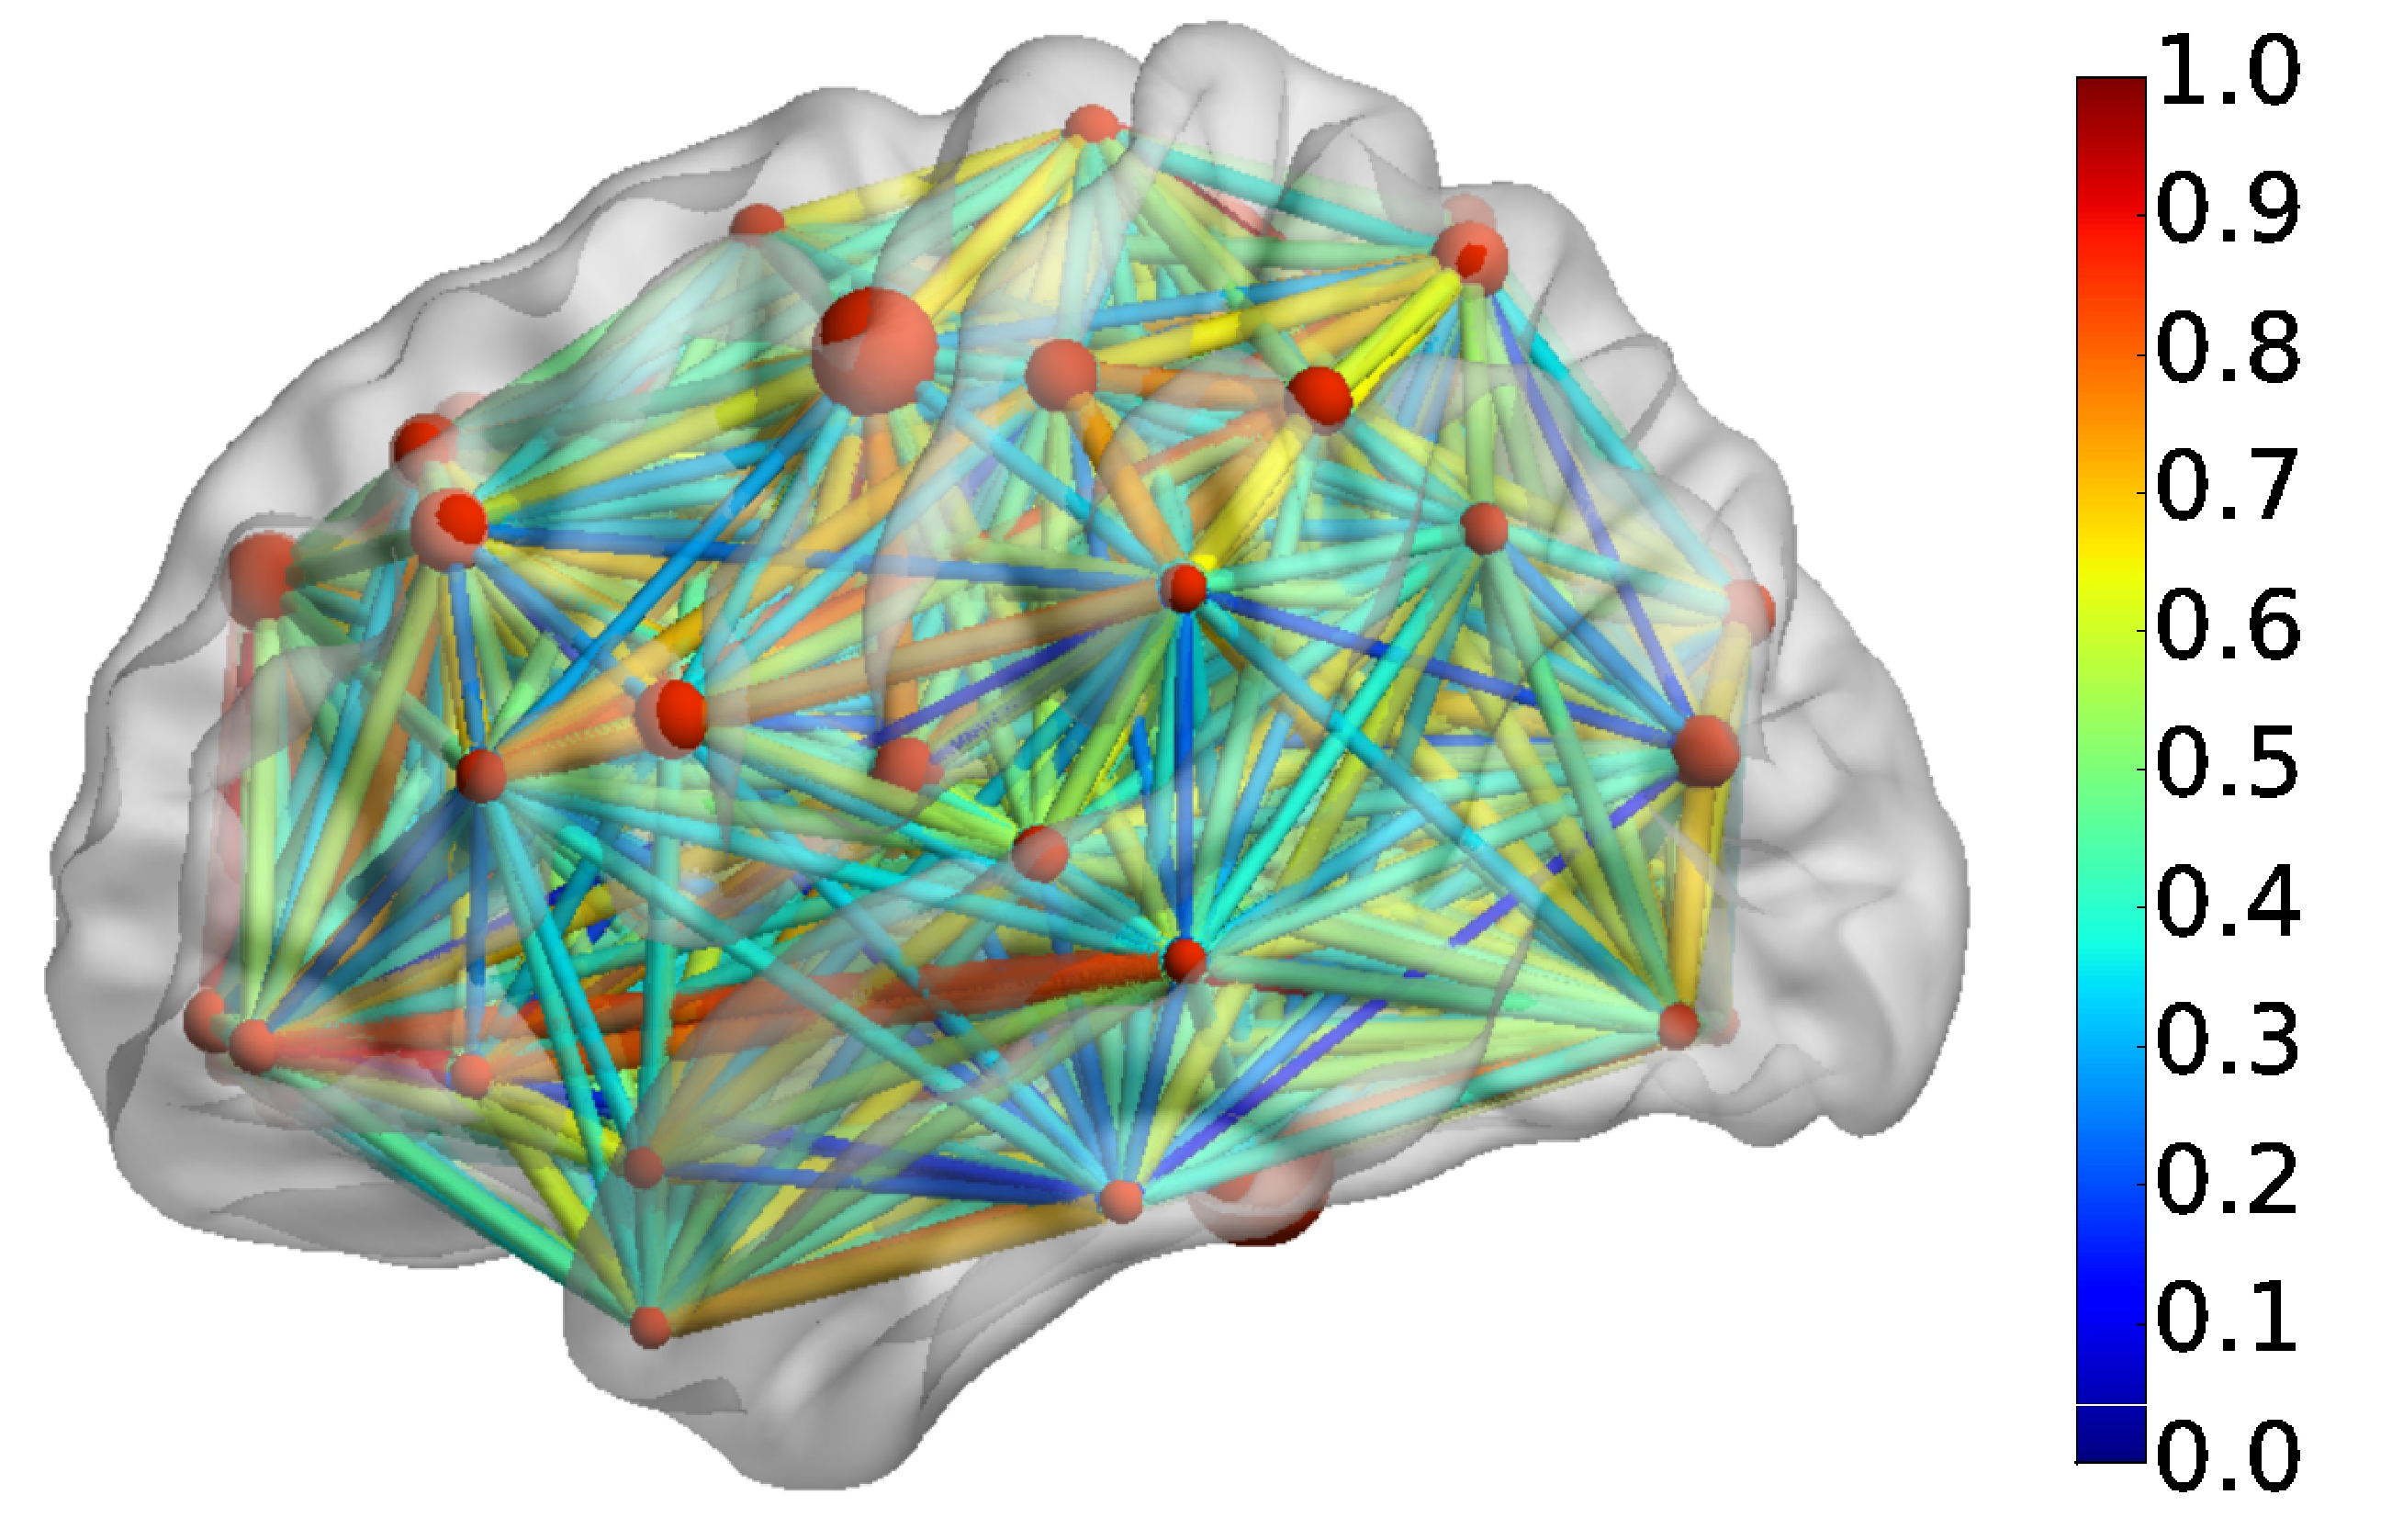
\includegraphics[width=0.40\textwidth]{Figures/FCM_brain.eps}
	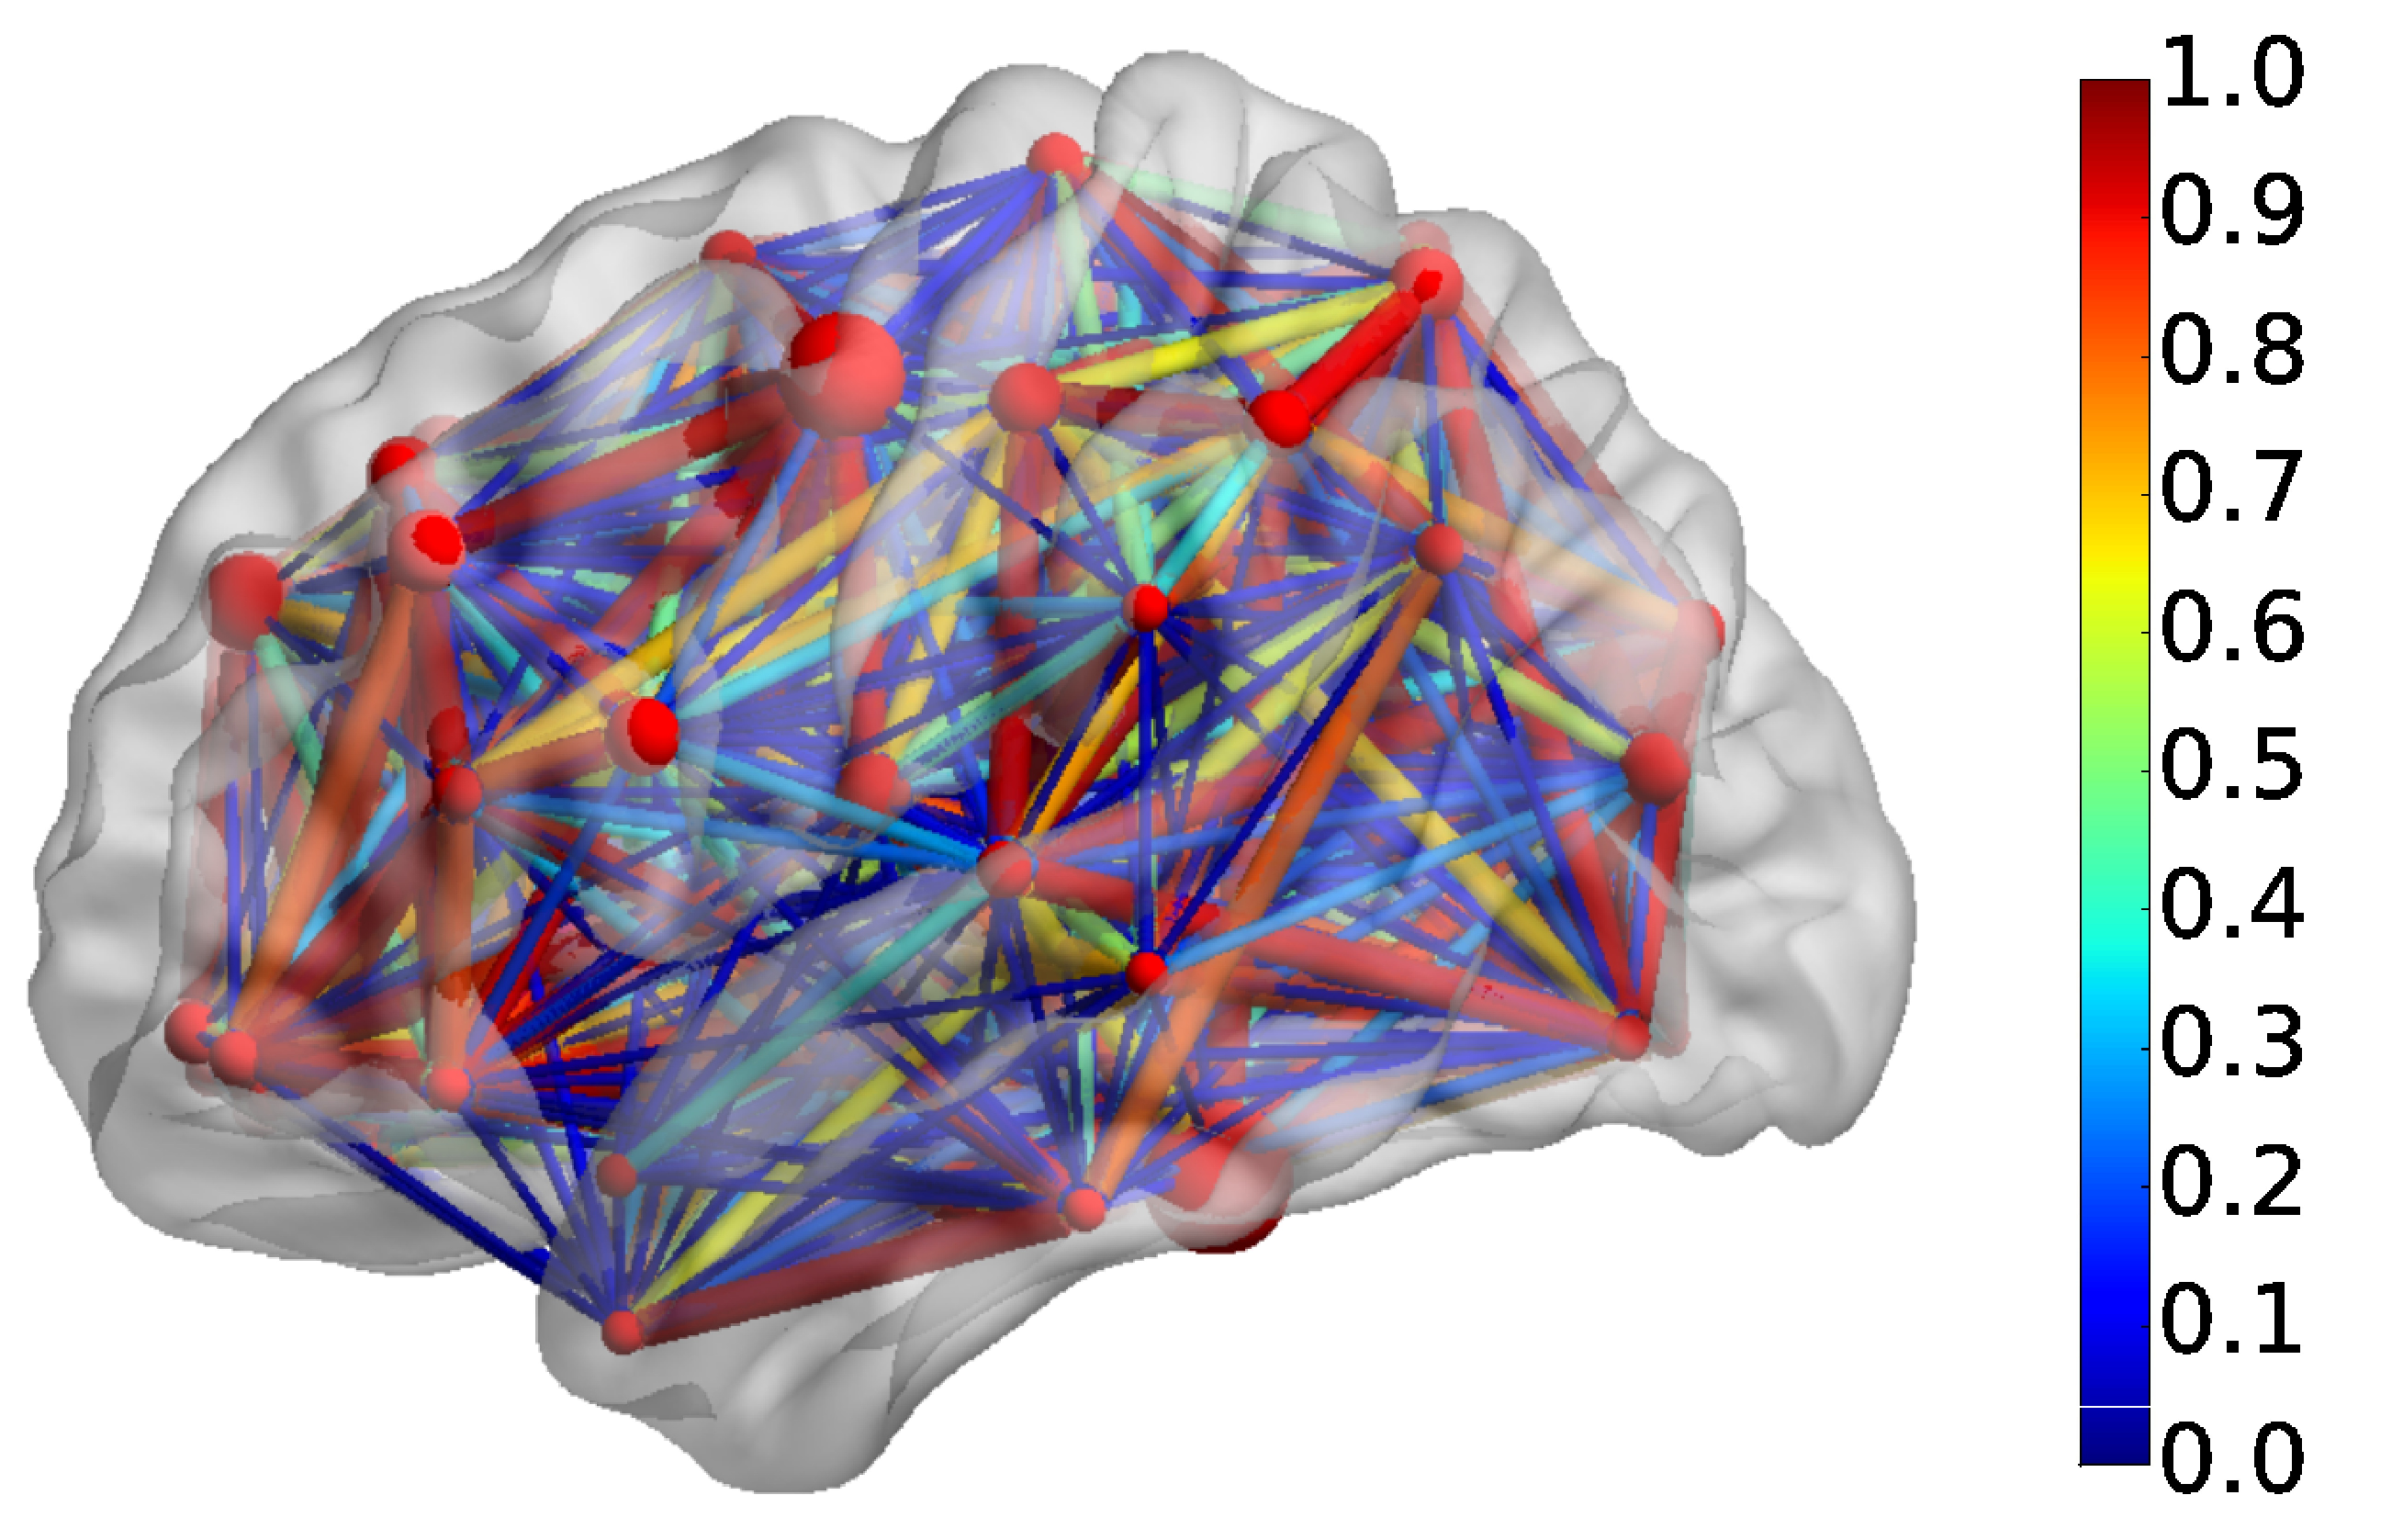
\includegraphics[width=0.40\textwidth]{Figures/ACM_brain.eps}

\end{frame}


\begin{frame}{2.The Brain Graph}
\centering
\footnotesize{FCM, (fMRI-BOLD) ~~~~~~~~~~~~  Adjacency Matrix (AM), r=0.55} 
	\includegraphics[width=0.38\textwidth]{Figures/cor_FCM_exp.eps} 
	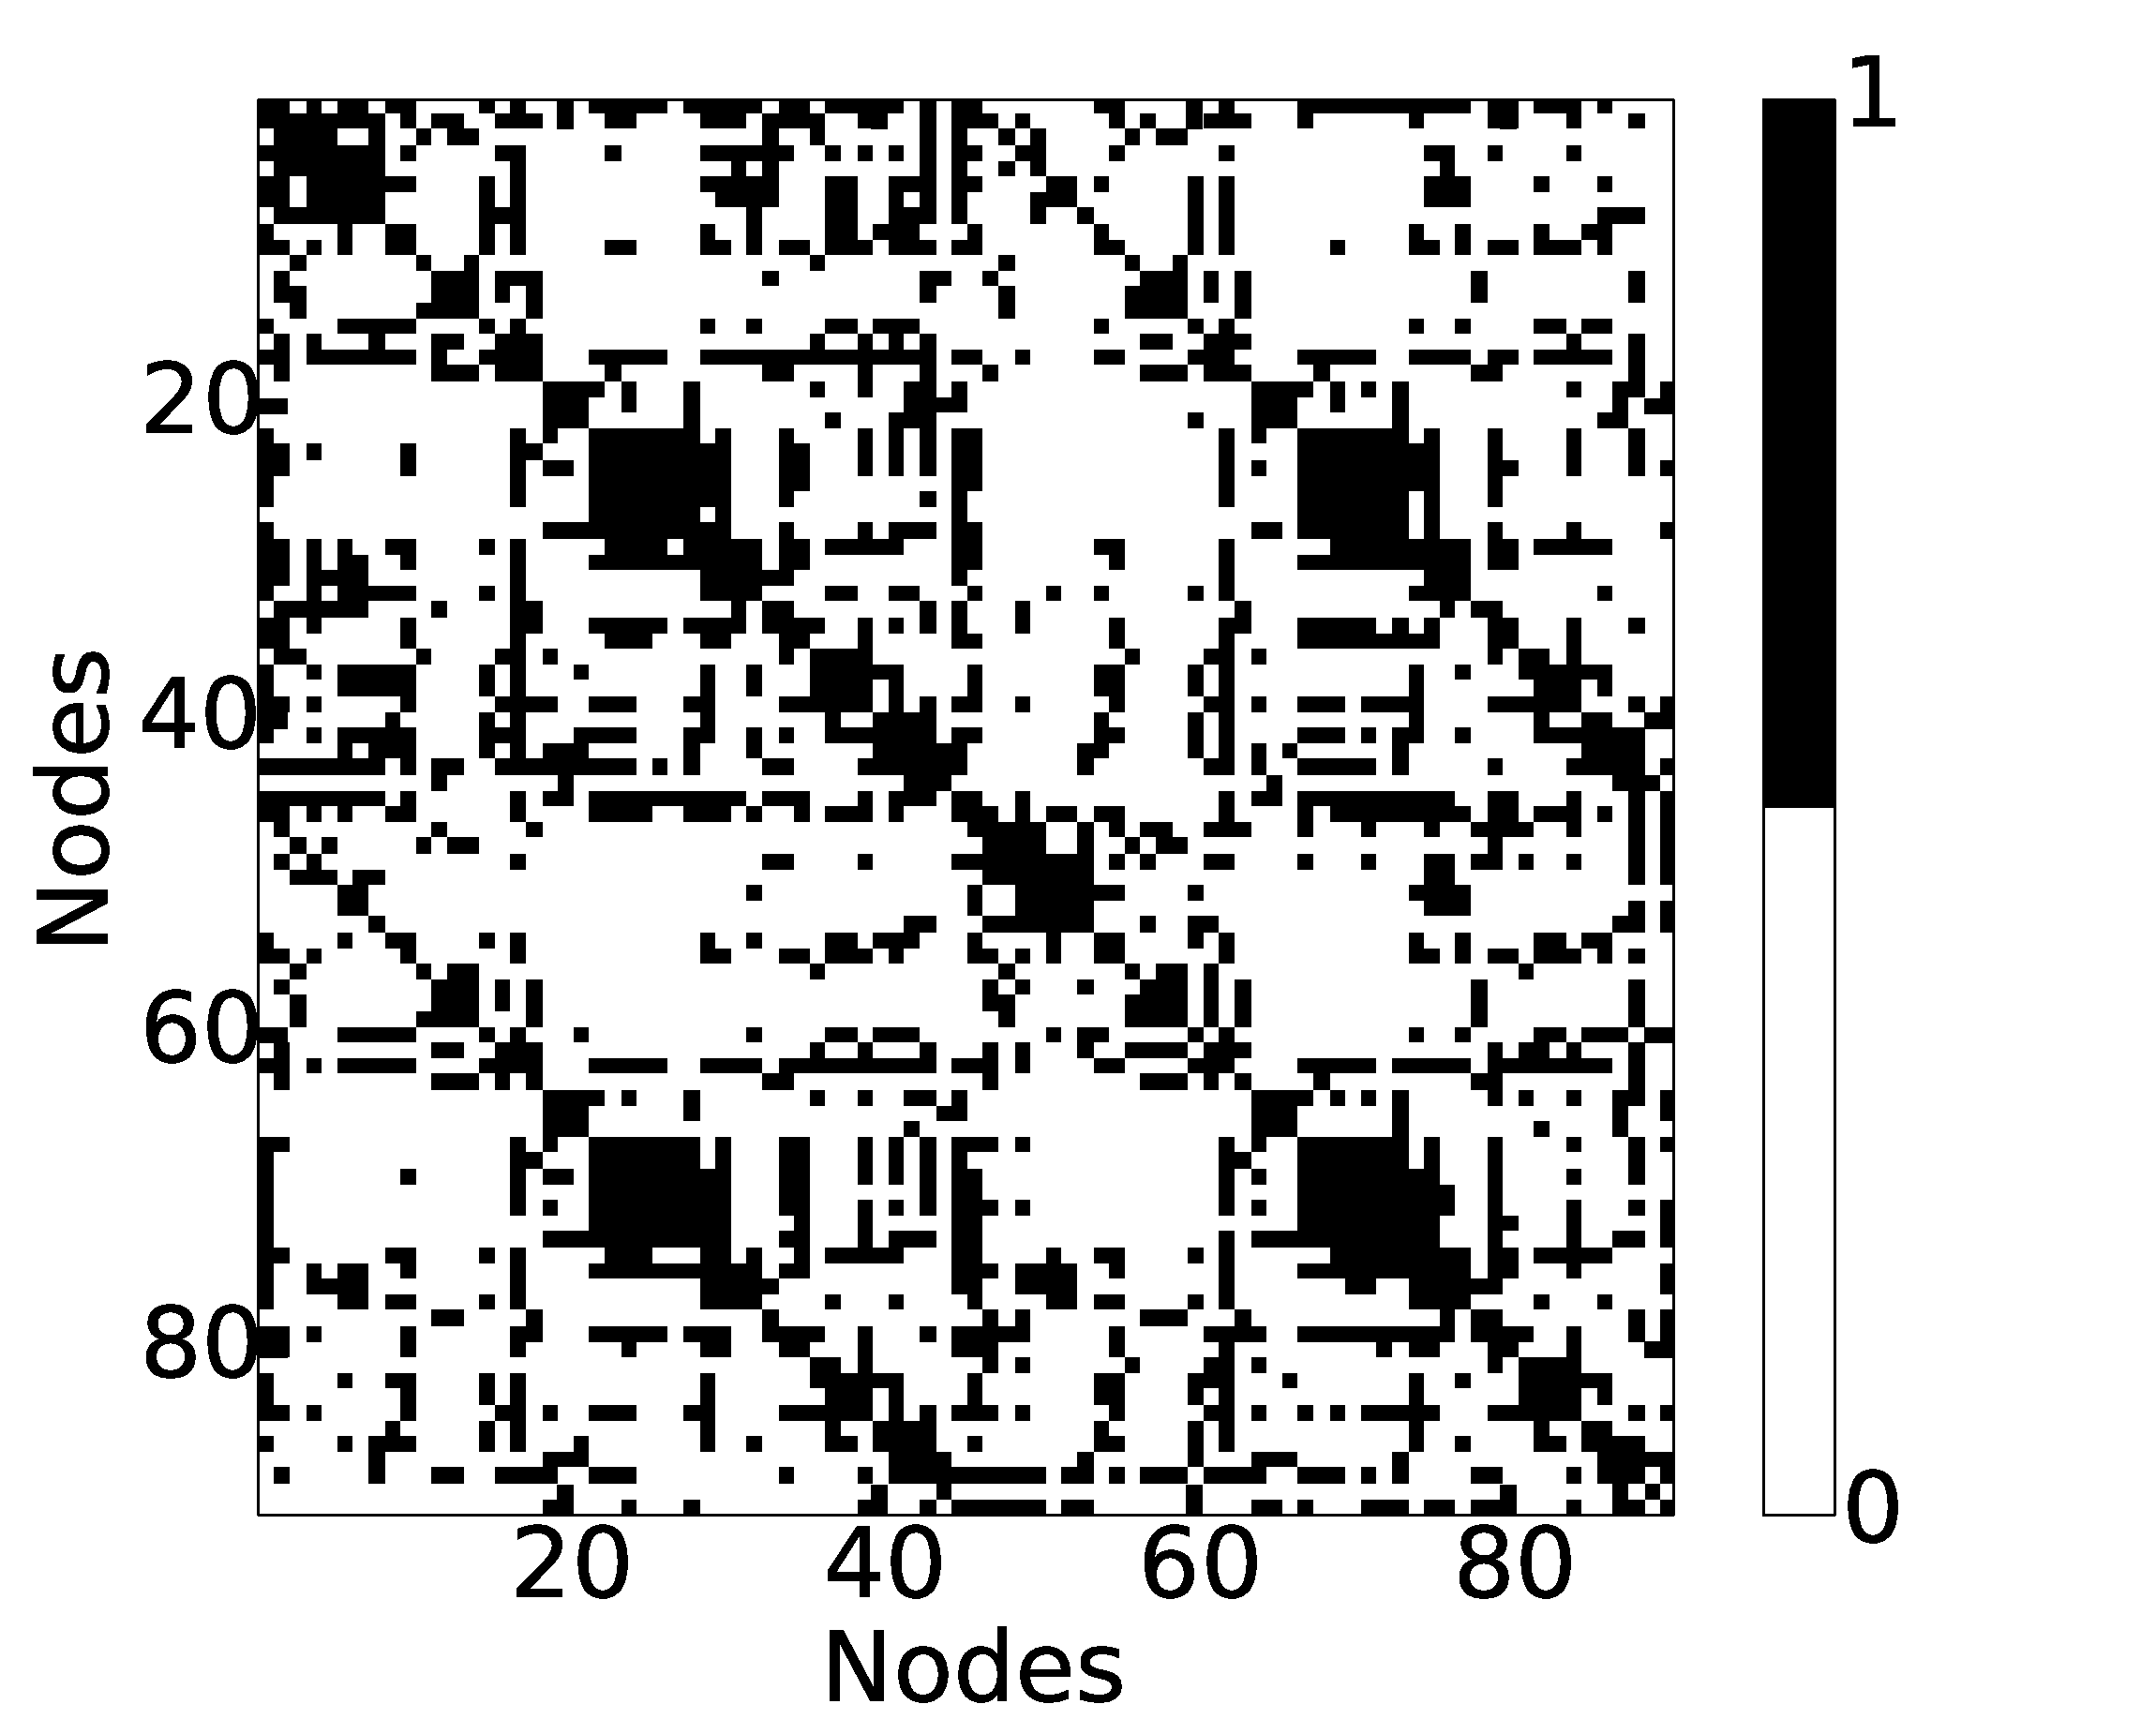
\includegraphics[width=0.38\textwidth]{Figures/Sample_Adj.eps} 
	
	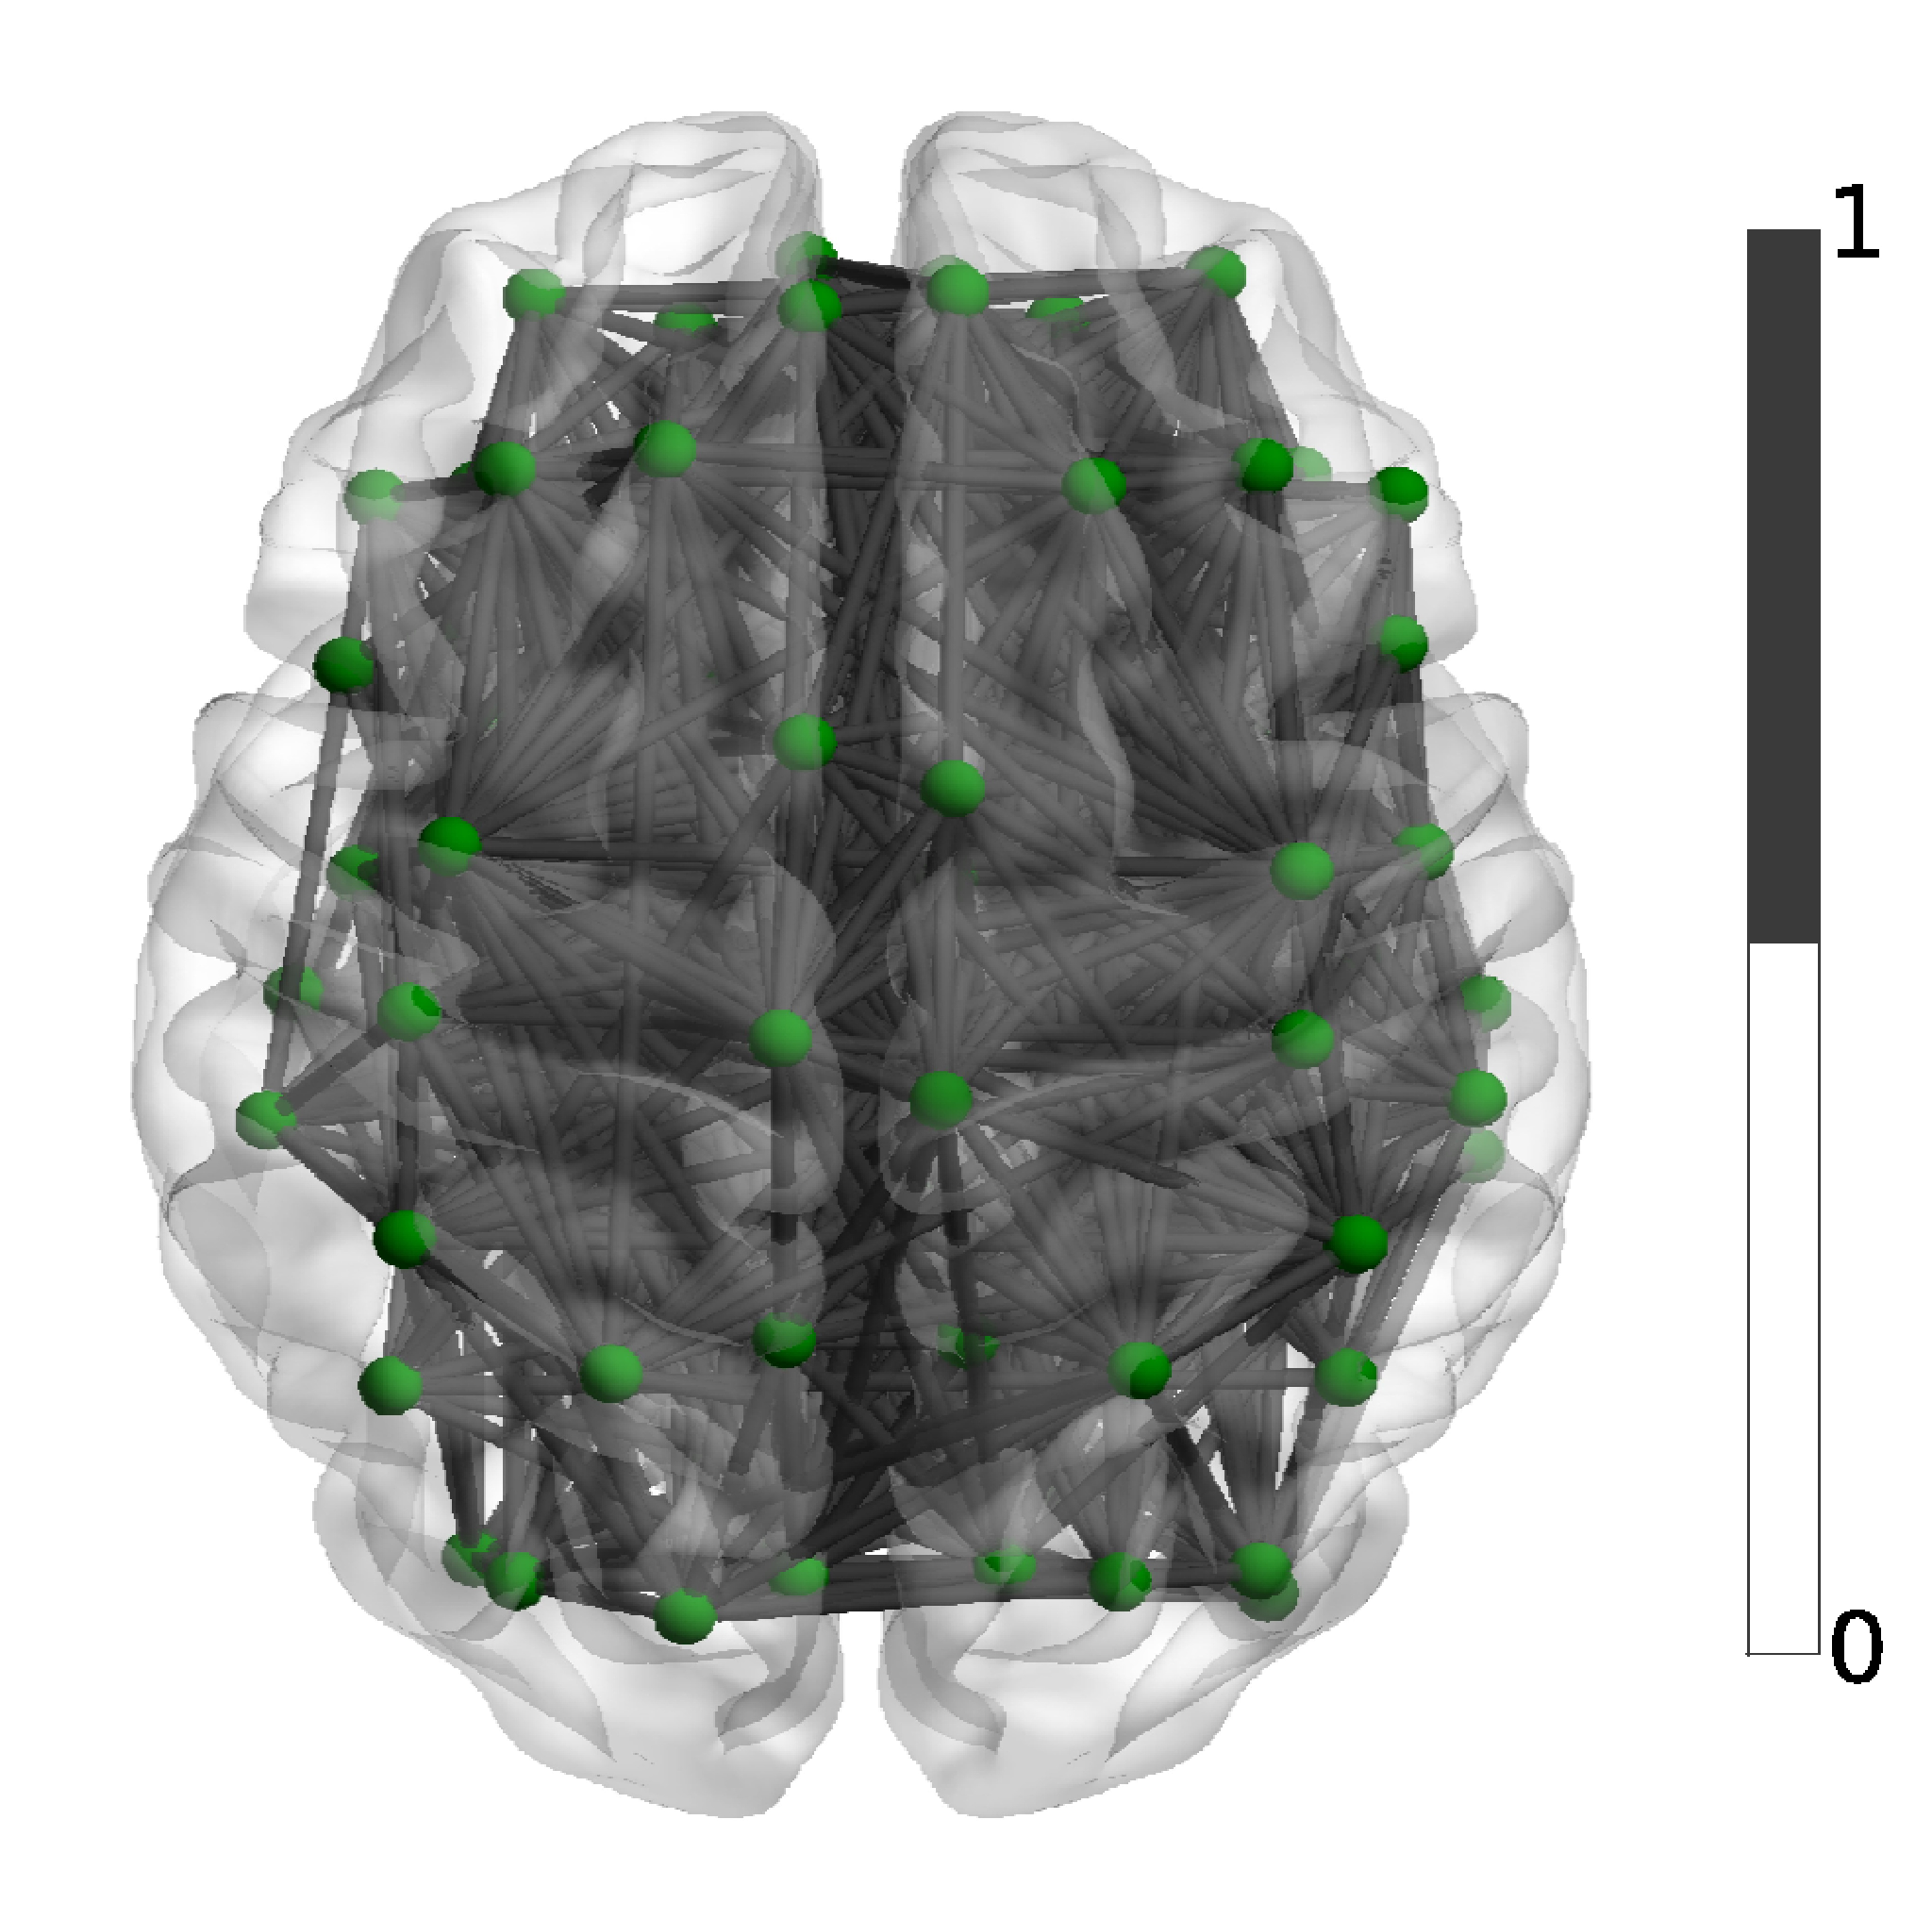
\includegraphics[width=0.30\textwidth]{Figures/Sample_Adj_brain.eps}  
    \includegraphics[width=0.30\textwidth]{Figures/brain_graph.png}      

\end{frame}


\begin{frame}{3.Randomization Methods}
	\begin{table}[h]
		\begin{center}
\caption[Abbreviations of Randomization Methods]{Abbreviations for the brain graph and the randomly constructed graphs }
\begin{tabular}{ l | c | r }
  Abbreviation & Description & method \\
  \hline  \hline                     
  $R_{BG}$ & the brain graph               & \textsc{NetworkX}  \\ \hline
  $R_{ER}$ & Erd\H{o}s-R\'{e}nyi, G(N,L)   & \textsc{NetworkX} \\ \hline
  $R_{DES}$ & double-edge-swap             & \textsc{NetworkX} \\ \hline
  $R_{PDD}$ & preserved-degree-distribution& \textsc{BCT} 	 \\ \hline  
  $R_{CM}$ & configuration model       	   & \textsc{NetworkX} \\ \hline
  $R_{PR}$ & partial randomization         & \textsc{BCT} 	 \\ \hline  
  \hline  
\end{tabular}
\label{table:Abbreviations of Randomization Methods}
		\end{center}
	\end{table}	

\end{frame}


\begin{frame}{3.The Randomization Methods}

\footnotesize{$R_{ER}$, Erd\H{o}s-R\'{e}nyi-Type Randomization, $G(N,L)$} 

($P$ : a binomial distribution for number of edges per node) 

	\includegraphics[width=0.33\textwidth]{Figures/f1.png}  
	\includegraphics[width=0.33\textwidth]{Figures/f2.png} 
    \includegraphics[width=0.33\textwidth]{Figures/f3.png}


$ L = \binom {N} {2}P $

\end{frame}


\begin{frame}{4.Network Characterizations}

	
	\begin{table}[h]
		\begin{center}
\caption[Statistical measures to characterize networks]{Statistical measures to characterize networks}
\begin{tabular}{ l  }
  Network Measures\\
  \hline  \hline                     
  		Network Density, $\kappa$ \\ \hline
  		Average Clustering Coefficient, $C$ \\ \hline
  		Transitivity, $T$ \\ \hline
  		Connected Components \\ \hline  
  		Small-Worldness, $S$ \\ \hline
  		Global and Local Efficiency, $E$ and $E_{loc}$  \\ \hline
  		Degree Distribution, $p(k)$ \\ \hline
  \hline  
\end{tabular}
\label{table:Statistical measures to characterize networks}
		\end{center}
	\end{table}	
	

\end{frame}


\begin{frame}{4.Network Characterizations}

{Average Clustering Coefficient, $C = \frac{1}{n} \sum\limits_{i\epsilon N}C_i = \frac{1}{n}\sum\limits_{i\epsilon N} \frac{2t_i}{k_i(k_i -1)}$} 
\break
\break
\break
\footnotesize{FCM related graphs ~~~~~~~~~~~~~ ACM related graphs}
	\centering	
	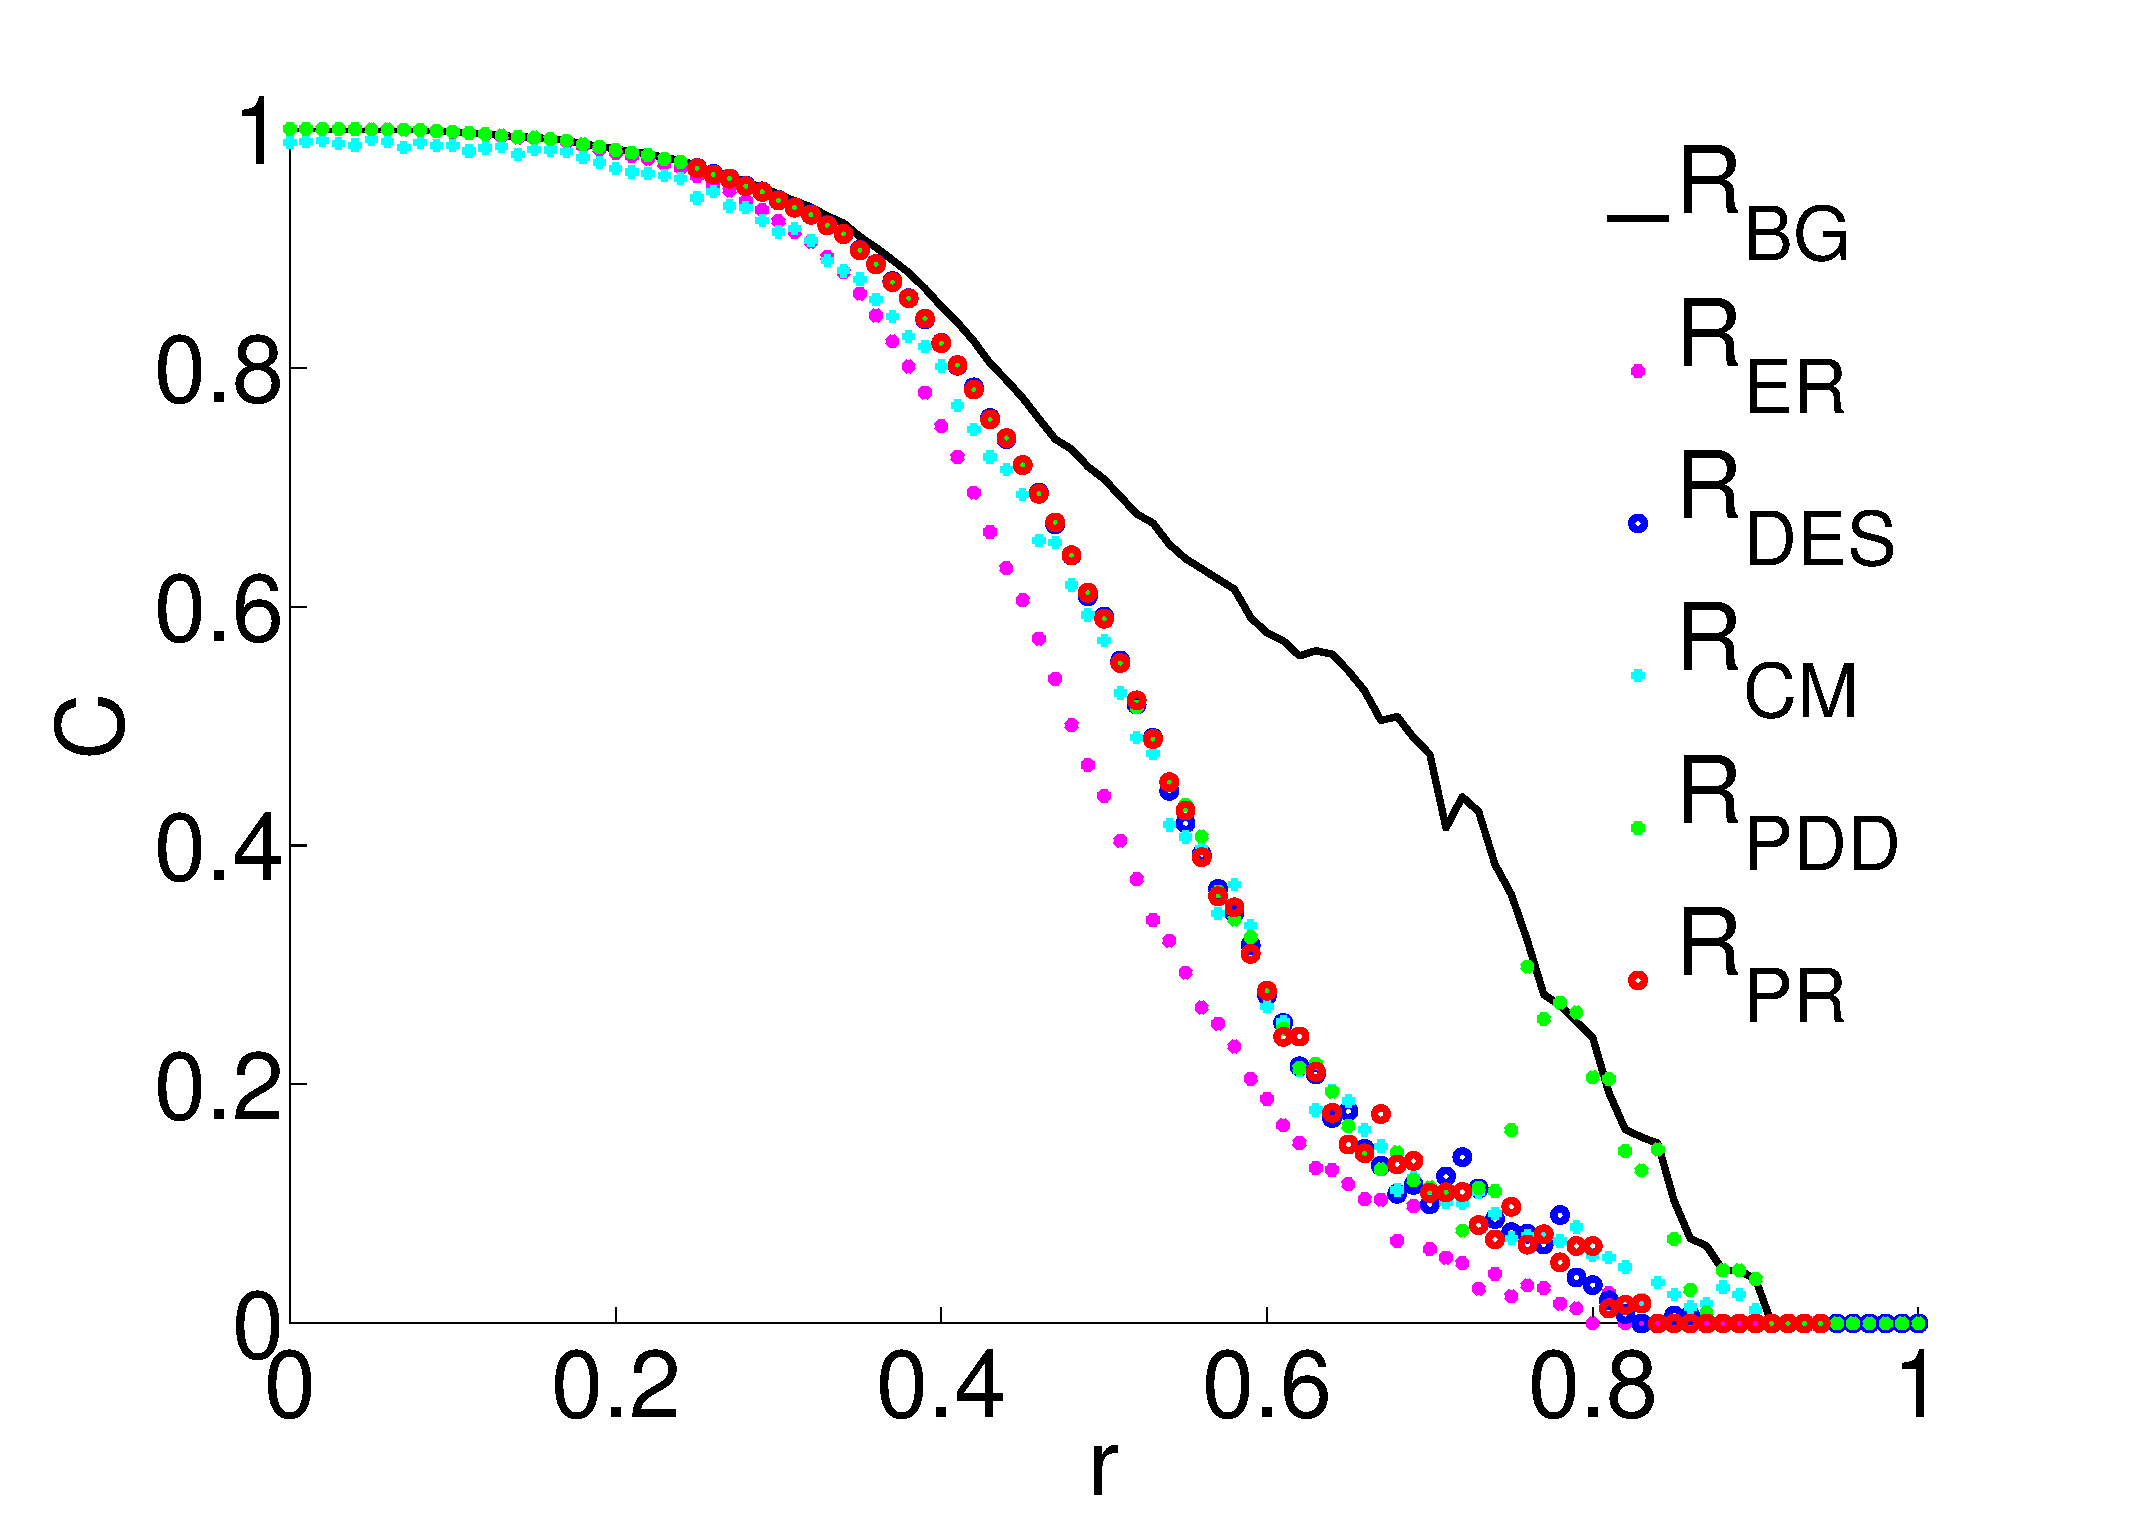
\includegraphics[width=0.40\textwidth]{Figures/Clustering_Coefficient_Fnc.eps}
	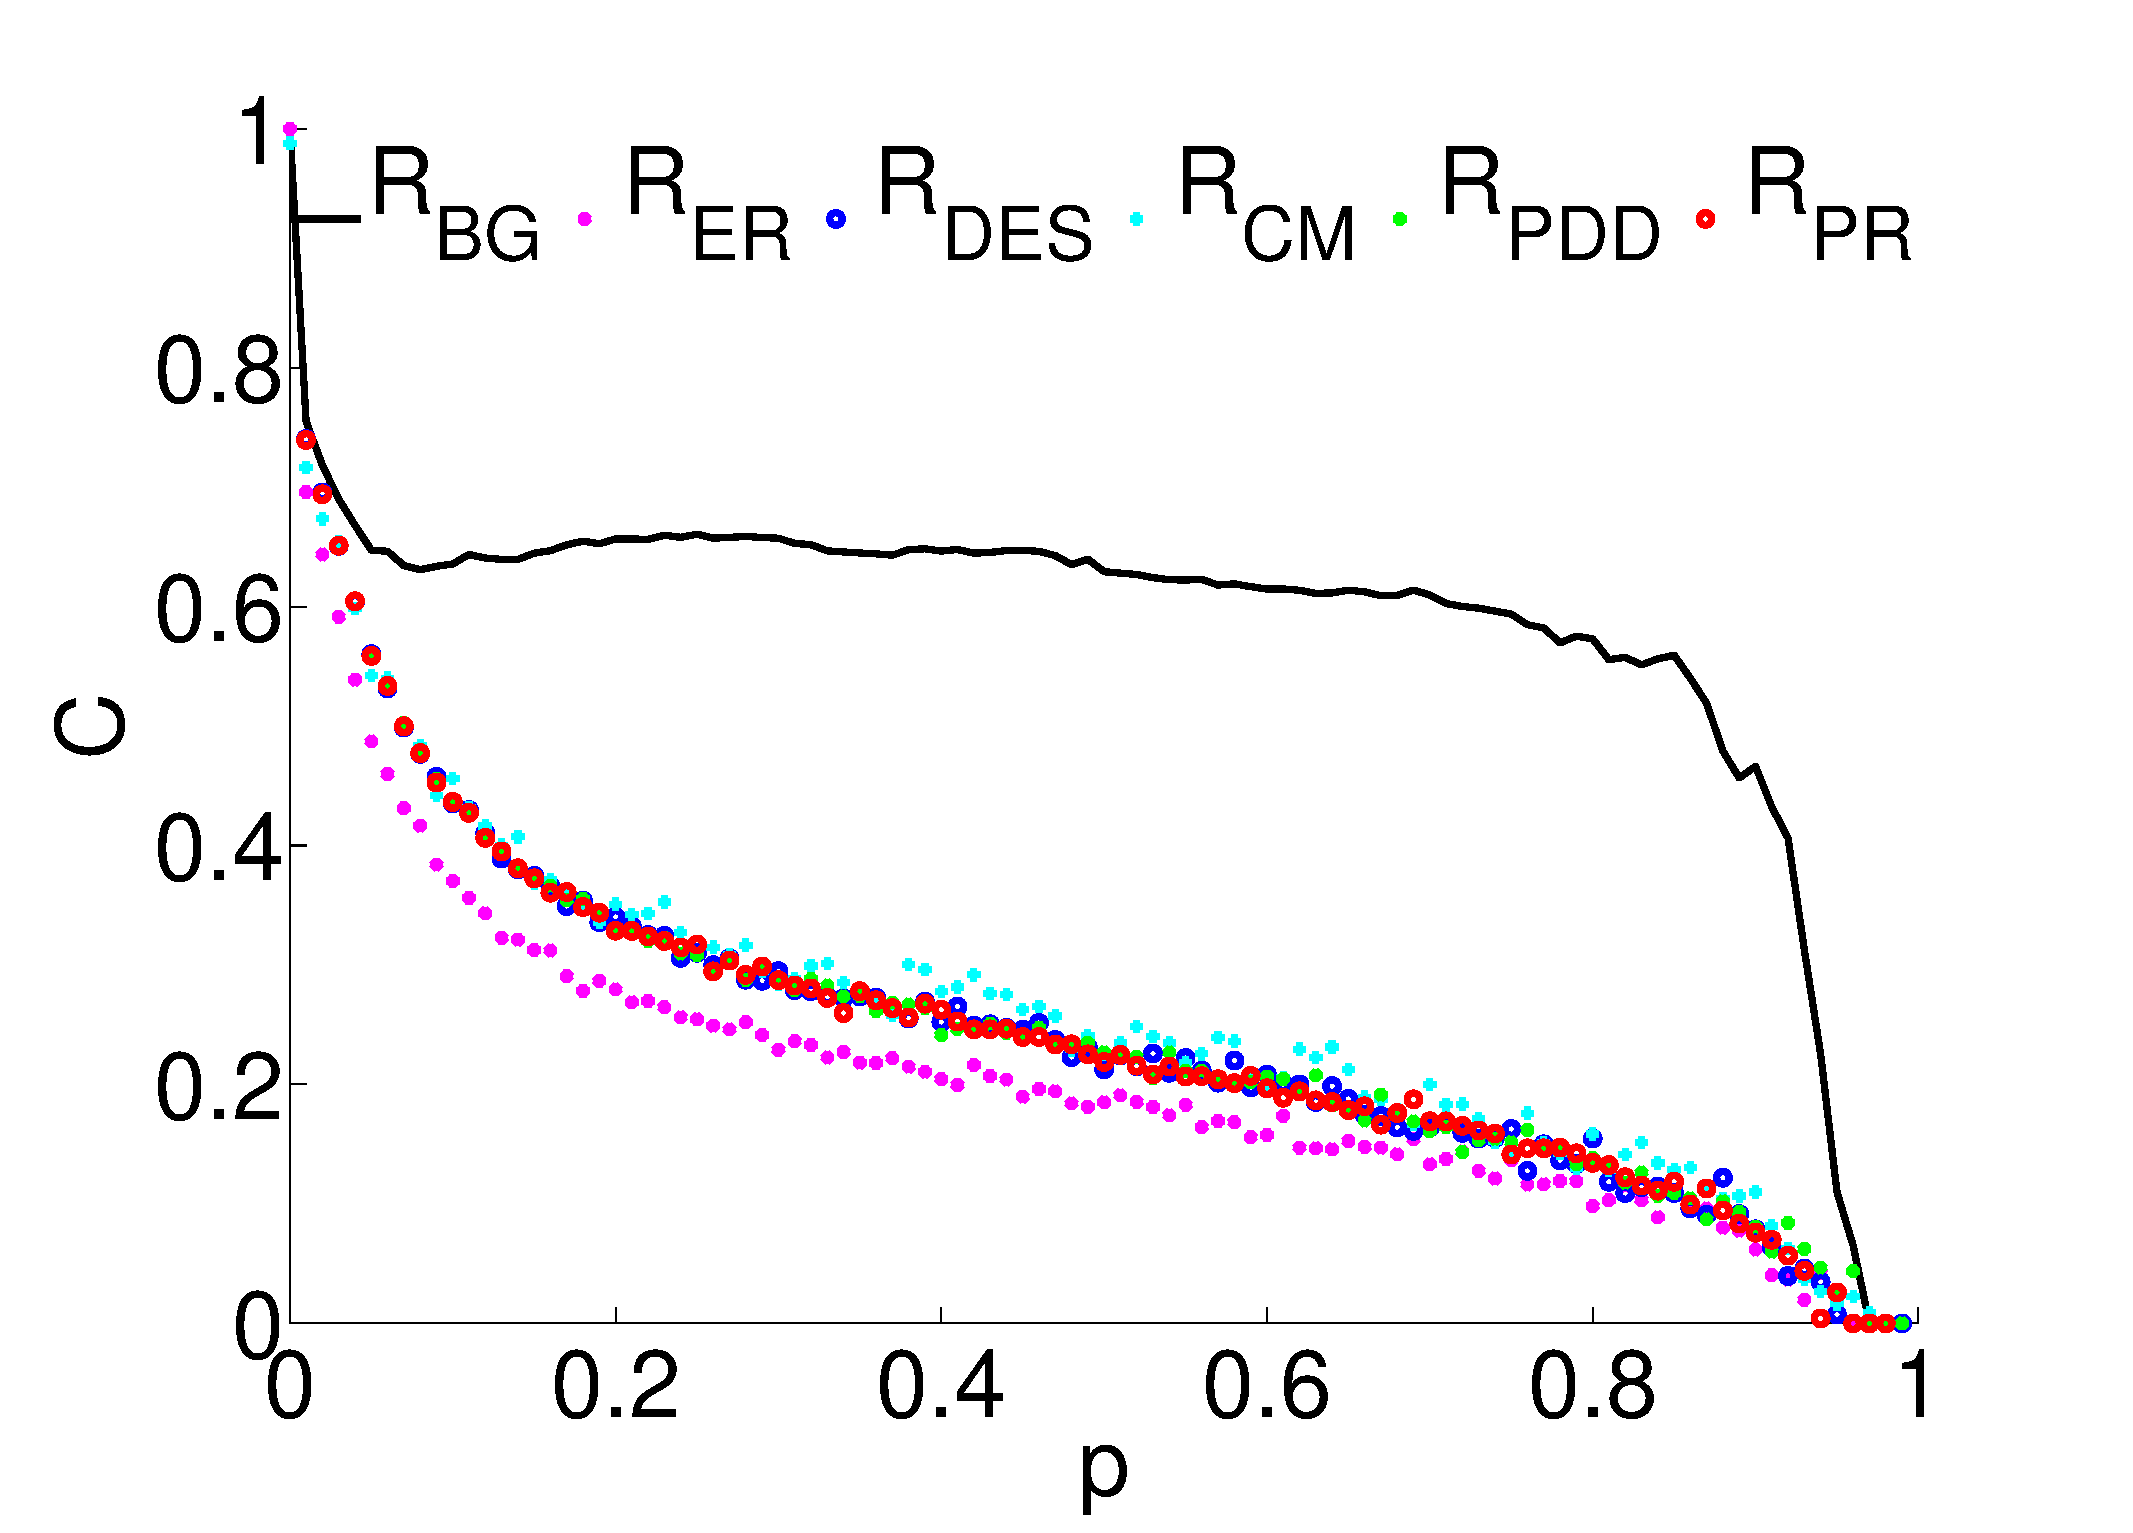
\includegraphics[width=0.40\textwidth]{Figures/Clustering_Coefficient_Stru.eps} 
\end{frame}


\begin{frame}{5.Neuronal Activity Model}
\footnotesize{FitzHugh-Nagumo Oscillations, Network Dynamics }

\begin{subequations}
 \begin{align}\dot{x_i} = \tau \left( y_i + \gamma x_i - \frac{x_i^3}{3} \right) -c \sum_{j=1}^N a_{ij}x_j(t - \Delta t_{ij}) +Dn_x \label{eqn: frobenius 3}\\  \dot{y_i} = -\frac{1}{\tau} (x_i - \alpha + b y_i  ) +Dn_y \label{eqn: frobenius 18}  , \end{align} 
\end{subequations}

  \centering
	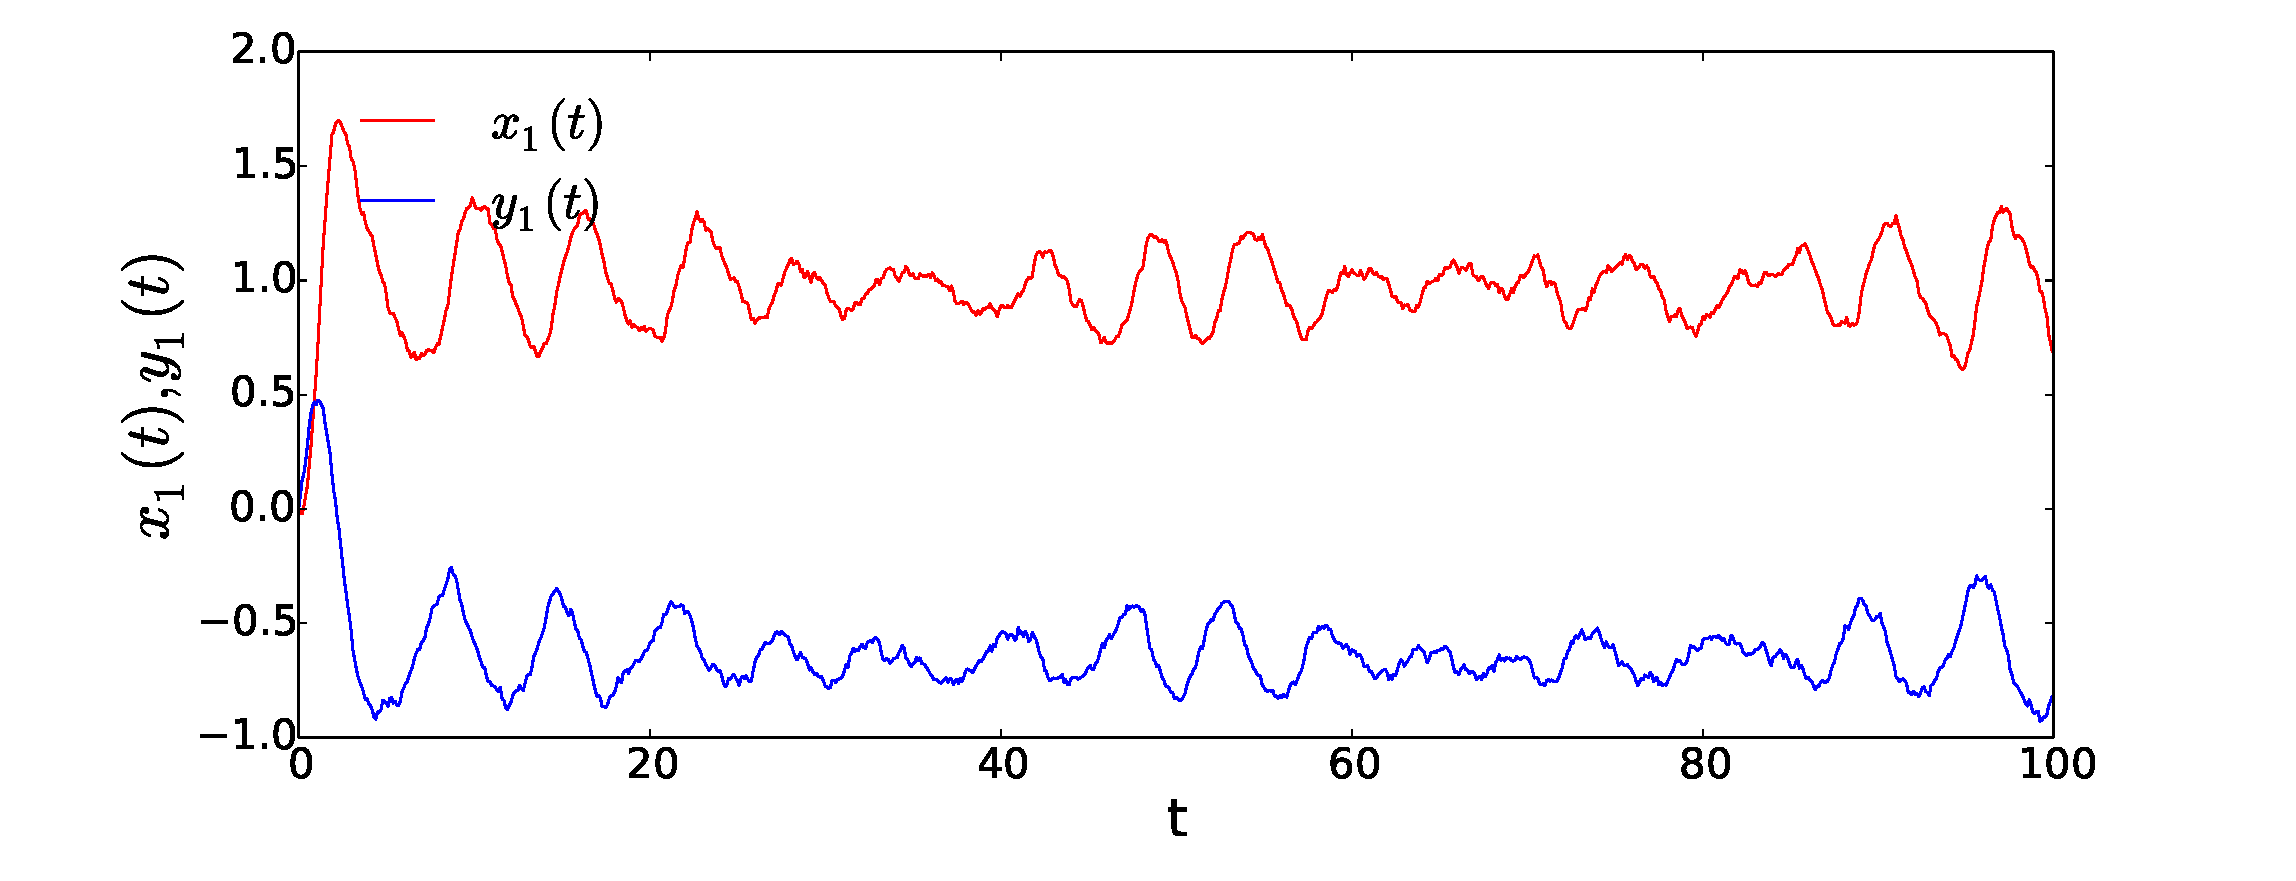
\includegraphics[width=0.8\textwidth, height=2.5cm]{Figures/FHN_time_1.eps} \\
 	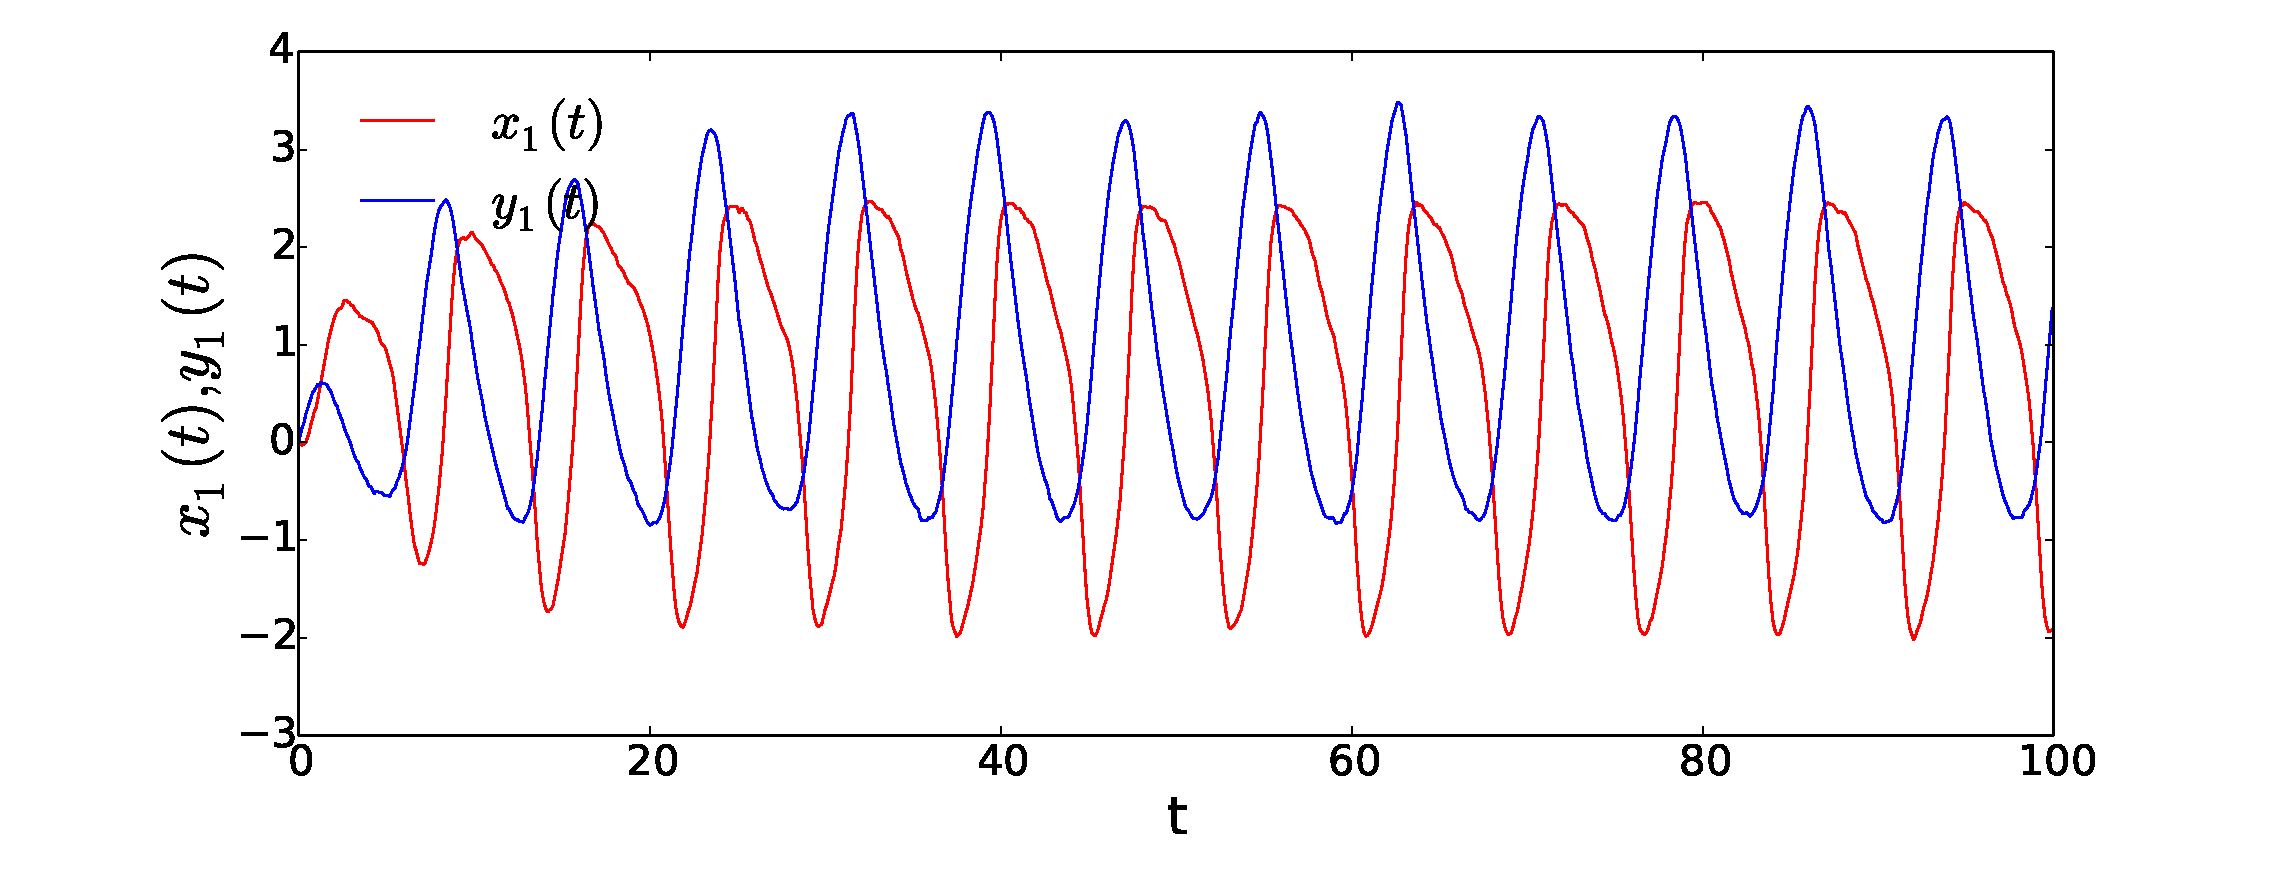
\includegraphics[width=0.8\textwidth, height=2.5cm]{Figures/FHN_time_2.eps}

\end{frame}

\begin{frame}{6.BOLD Activity Model}
\footnotesize{Balloon-Windkessel Hemodynamic Model}

\centering
\includegraphics[width=0.7\textwidth]{Figures/BOLD_Hemo.eps}

\begin{itemize}
 \item neuronal activity  $\Rightarrow$ regional changes in surrounding
 \item CBV, CBF, $O_2$-level, $Hb$ and $dHB$ level in capillaries 
 \item Friston et. al.: mediating between non-linear time-series and BOLD activity 
\end{itemize}

\end{frame}


\begin{frame}{7.Results}

Parameter Analysis
\begin{itemize}
\item  $c$, the coupling strength (FHN network model) 
\item  $v$, the axonal propagation velocity, $\Delta t_{ij} = d_{ij}/v$ (FHN network model)
\item  $r$ or $p$, threshold or probability (network topology)

\end{itemize}

\end{frame}


\begin{frame}{7.Results}
\footnotesize{Neuronal Activity Simulations of FCM Related Brain Graphs to fMRI-BOLD Data}

\break

	\centering
	 \includegraphics[width=0.35\textwidth]{Figures/cor_FCM_sim.eps} 
   	 \includegraphics[width=0.35\textwidth]{Figures/cor_FCM_exp.eps} 

 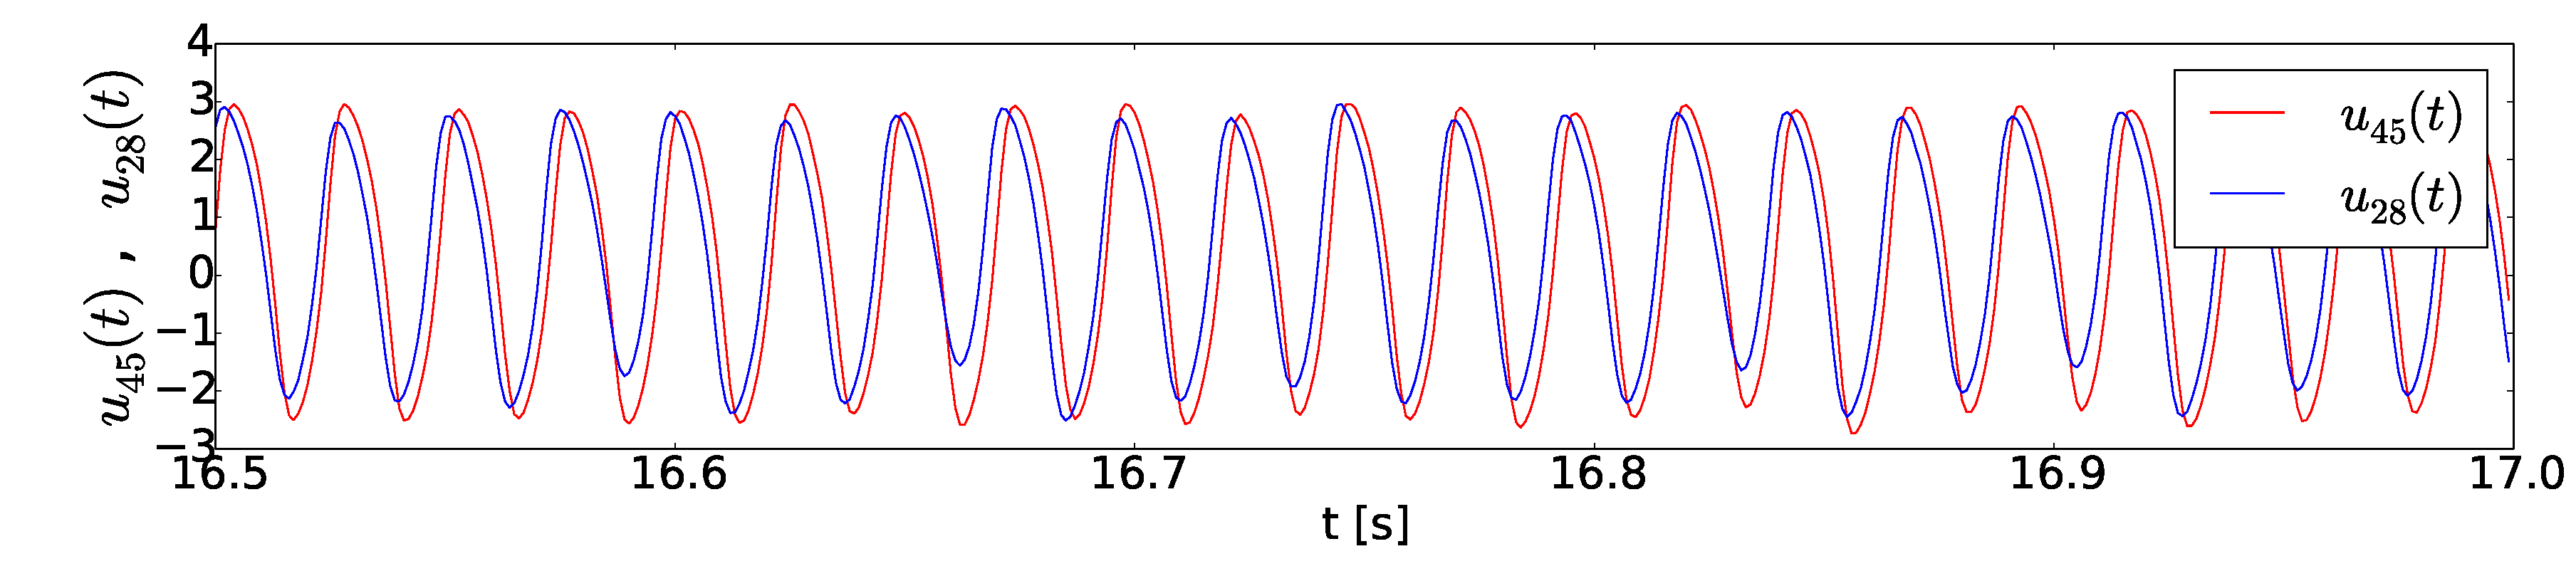
\includegraphics[width=0.7\textwidth]{Figures/cor_FCM_sim_no_best.eps} \\
 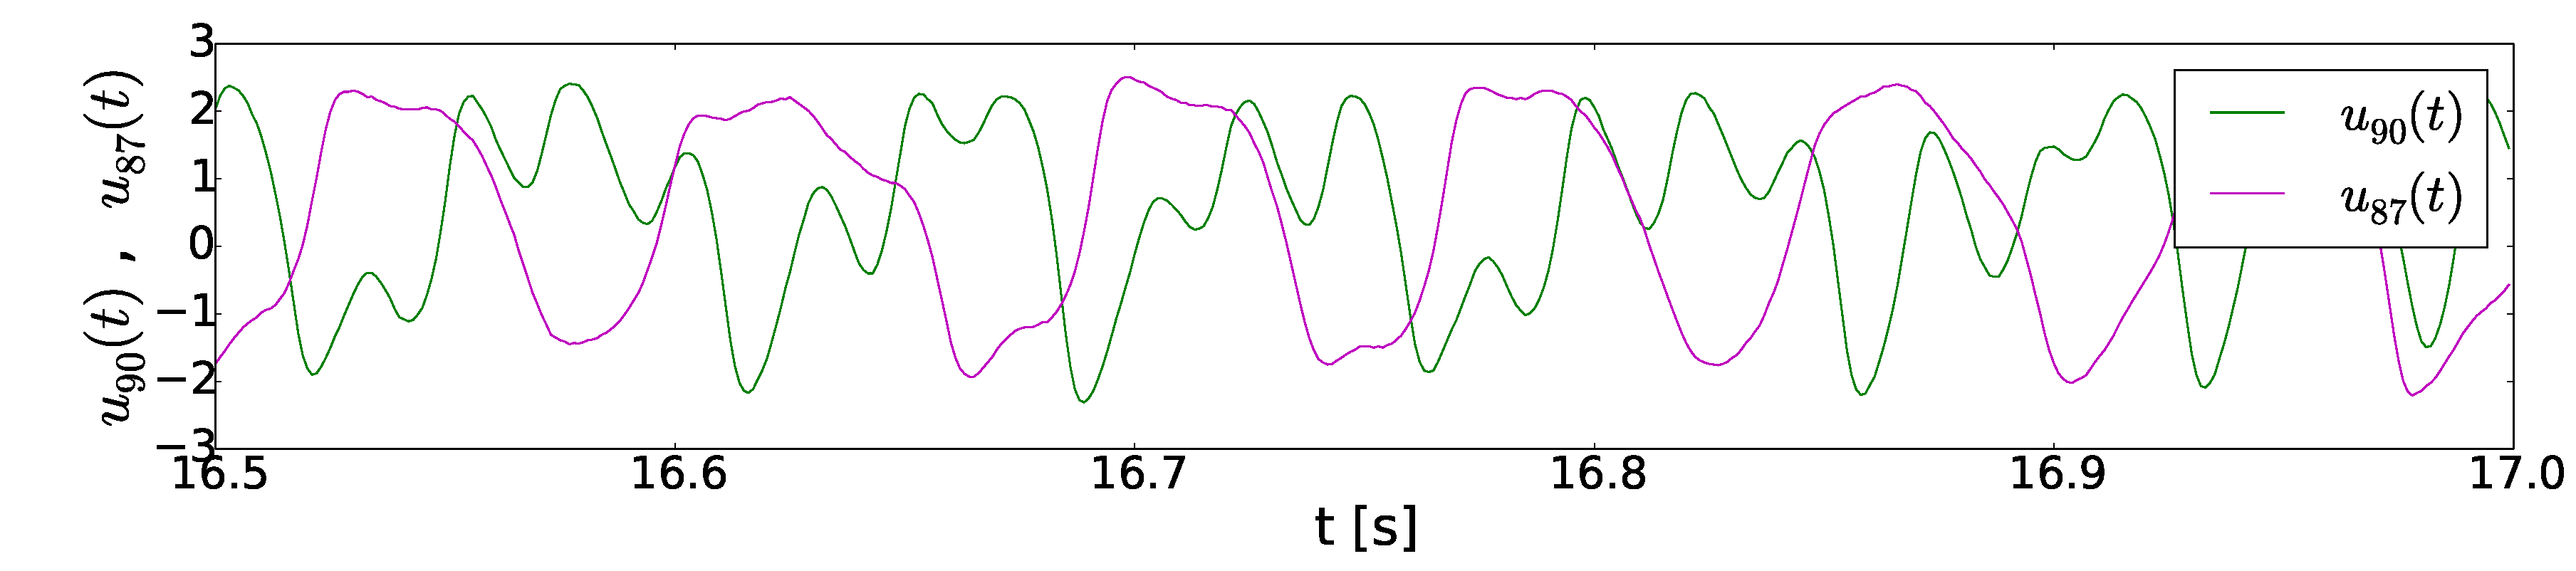
\includegraphics[width=0.7\textwidth]{Figures/cor_FCM_sim_no_worst.eps} 

\tiny{$c=0.2,~~ v=7 m/s, ~~ r=0.60, ~~ \rho_{e,s}=0.43$, ~~ $\rho_{45,28}=0.88$, ~~~~~~ $\rho_{90,87}=0.13$}

\end{frame}


\begin{frame}{7.Results}

\footnotesize{Comparing BOLD Simulations of Anatomical Brain Graphs to fMRI-BOLD Data} 
\break
	\centering
    \includegraphics[width=0.49\textwidth]{Figures/PA_BOLD_ACM_v_3.eps} 
    
 $v=3 m/s$   
    
\end{frame}



\begin{frame}{7.Results}
\footnotesize{Comparing BOLD Simulations of Anatomical Brain Graphs to fMRI-BOLD Data} 
\break
	\centering
	 \includegraphics[width=0.49\textwidth]{Figures/cor_BOLD_ACM_sim.eps} 
   	 \includegraphics[width=0.49\textwidth]{Figures/cor_FCM_exp.eps} 

$c=0.03, ~~~ v=3 m/s, ~~~ p=0.54, ~~~~, \rho_{e,s}=0.22$

\end{frame}


\begin{frame}{7.Results}
\footnotesize{Comparison of FCM Related Brain Graph to the Random Networks}
\begin{center}

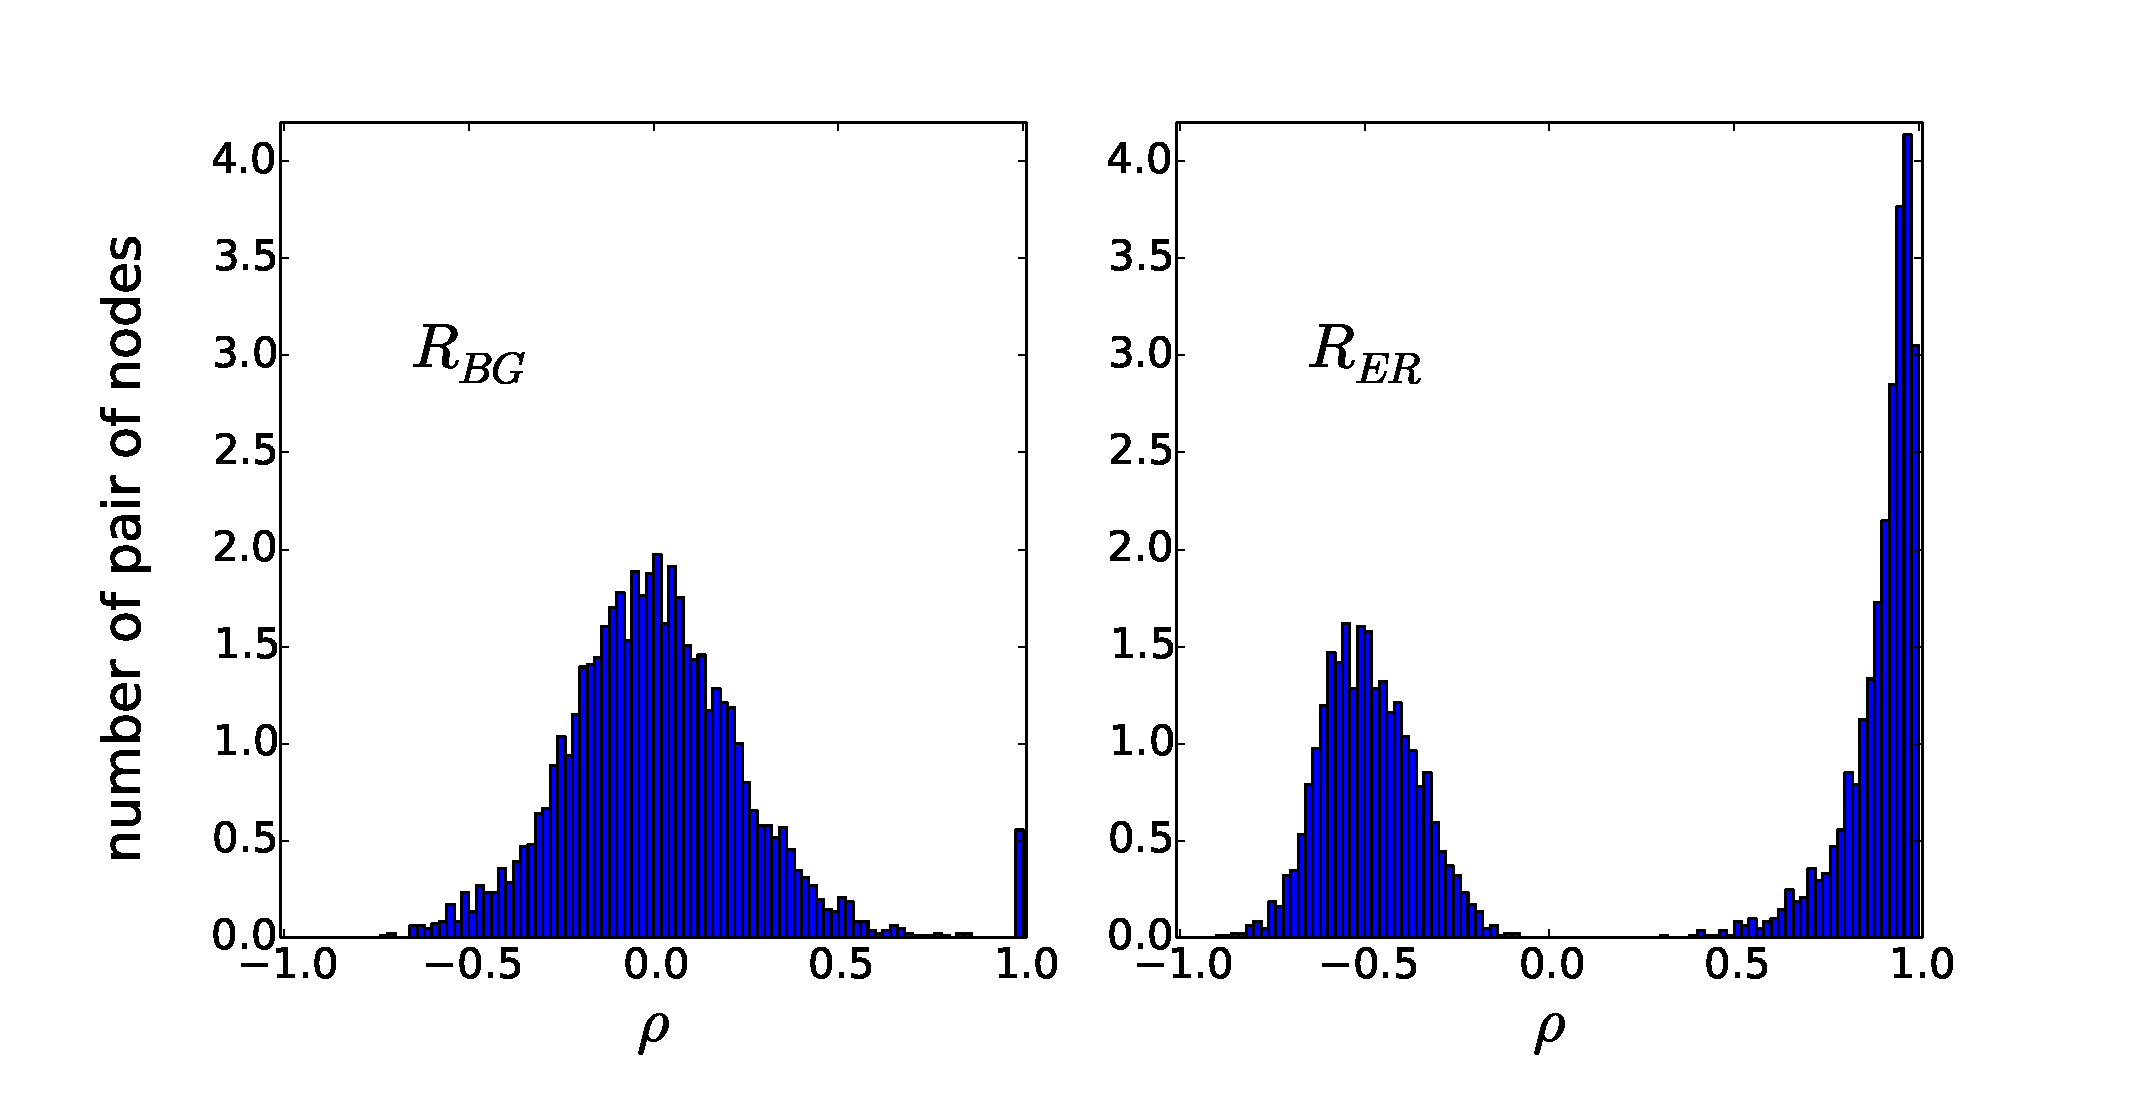
\includegraphics[width=8cm, height=3cm]{Figures/R_BG_R_ER_histo_1.eps} \\
\tiny{$r=0.61$,~~~$c=0.1$,~~~$v=7$ m/s} \\
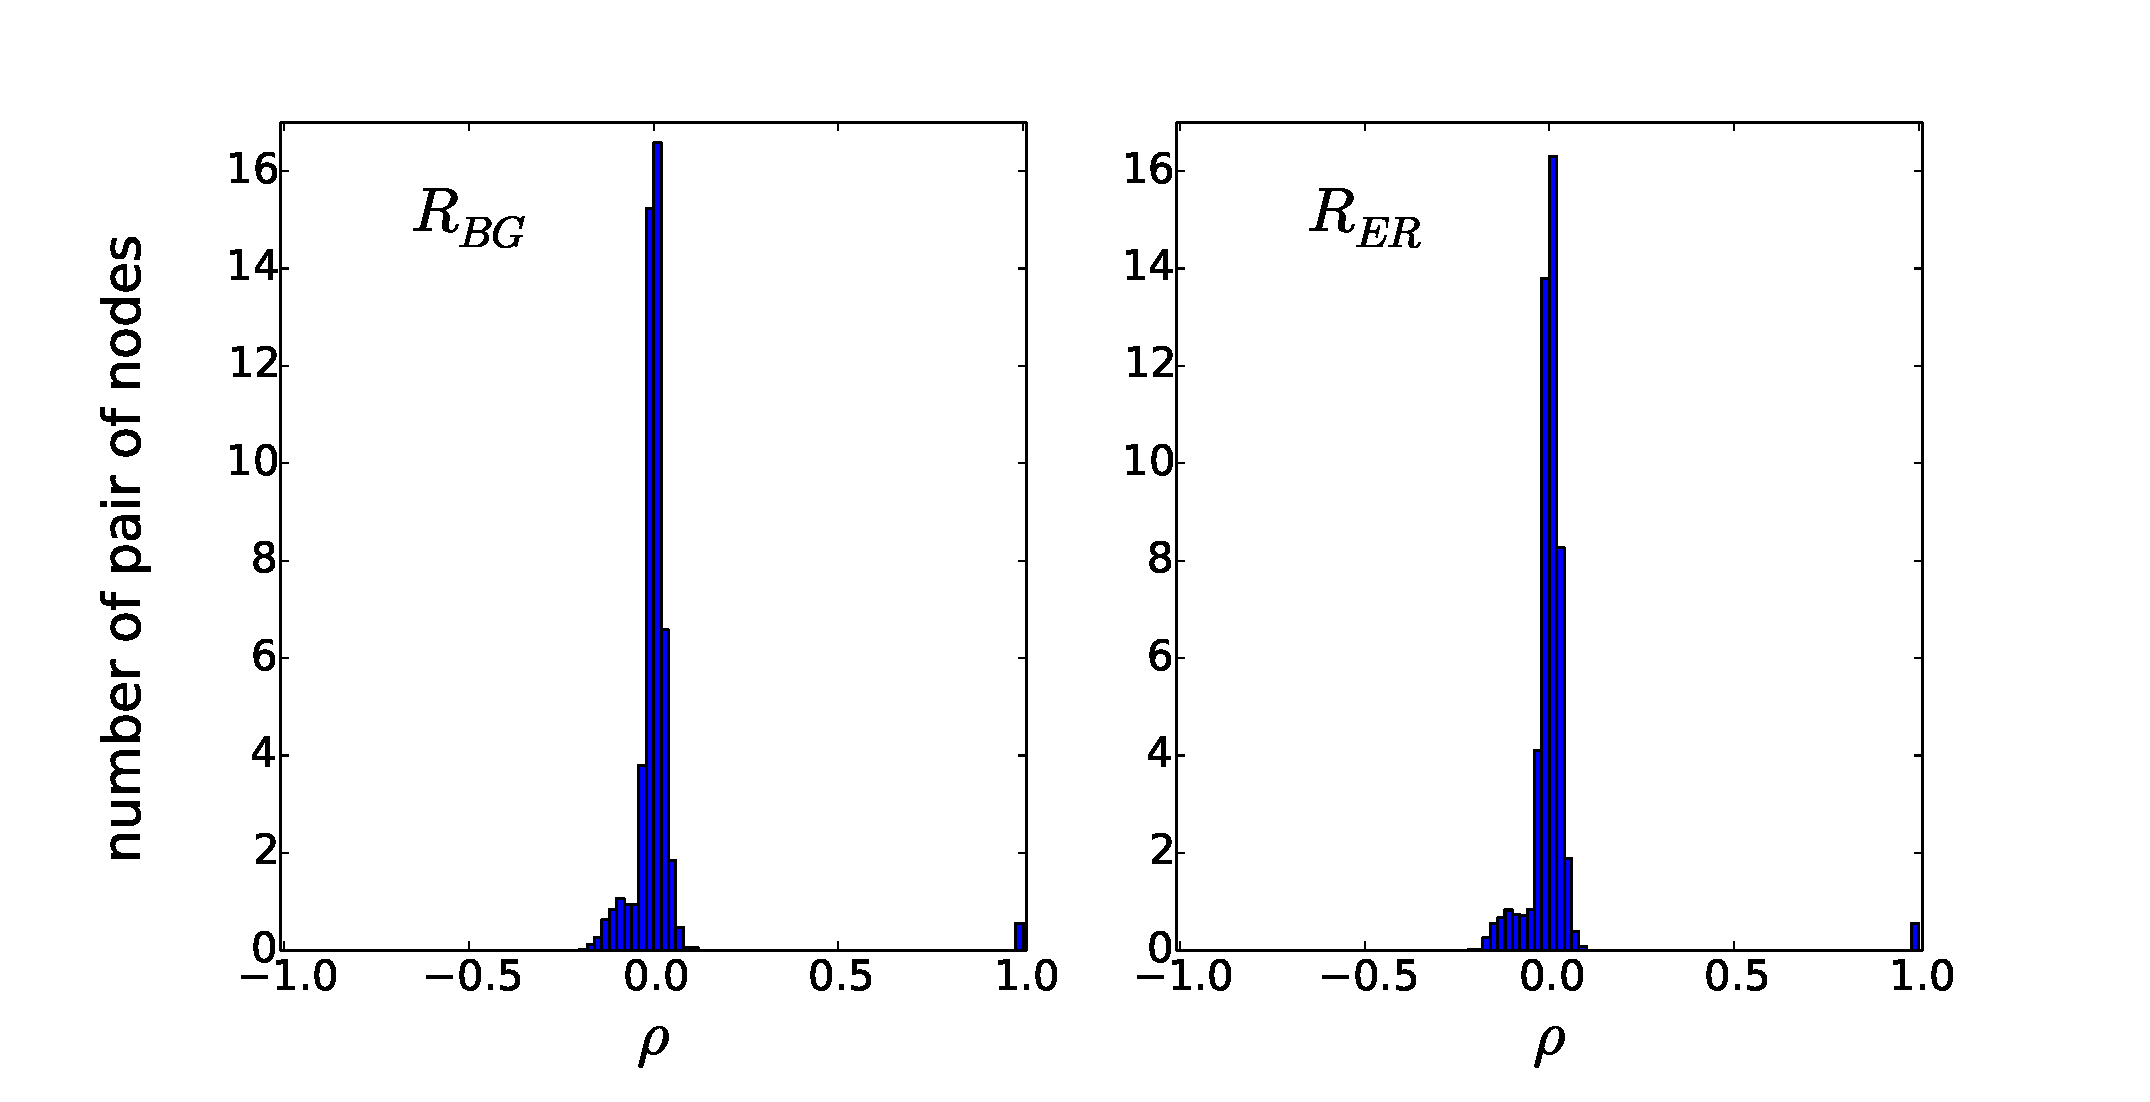
\includegraphics[width=8cm, height=3cm]{Figures/R_BG_R_ER_histo_2.eps} \\
\tiny{$r=0.60$,~~~$c=0.018$,~~~$v=7$ m/s}
\end{center}


\end{frame}





\begin{frame}{7.Results}
\footnotesize{Comparison of FCM Related Brain Graph to the Random Networks}
\centering
\includegraphics[width=0.6\textwidth]{Figures/R_BG_R_ER_PA.eps}\\
\tiny{$v=7$ m/s}

\end{frame}









\begin{frame}{Thanks}

\end{frame}



\begin{frame}{References}

\end{frame}


\begin{frame}{9.Discussion}

\end{frame}




\begin{frame}{3.The Randomization Methods}

\footnotesize{Erd\H{o}s-R\'{e}nyi-Type Randomization, $G(N,L)$} 

	\includegraphics[width=0.30\textwidth]{Figures/f1.png}  
	\includegraphics[width=0.30\textwidth]{Figures/f2.png} 
    \includegraphics[width=0.30\textwidth]{Figures/f3.png}
    
\footnotesize{Double-Edge-Swap Type Randomization, $k_i$}
	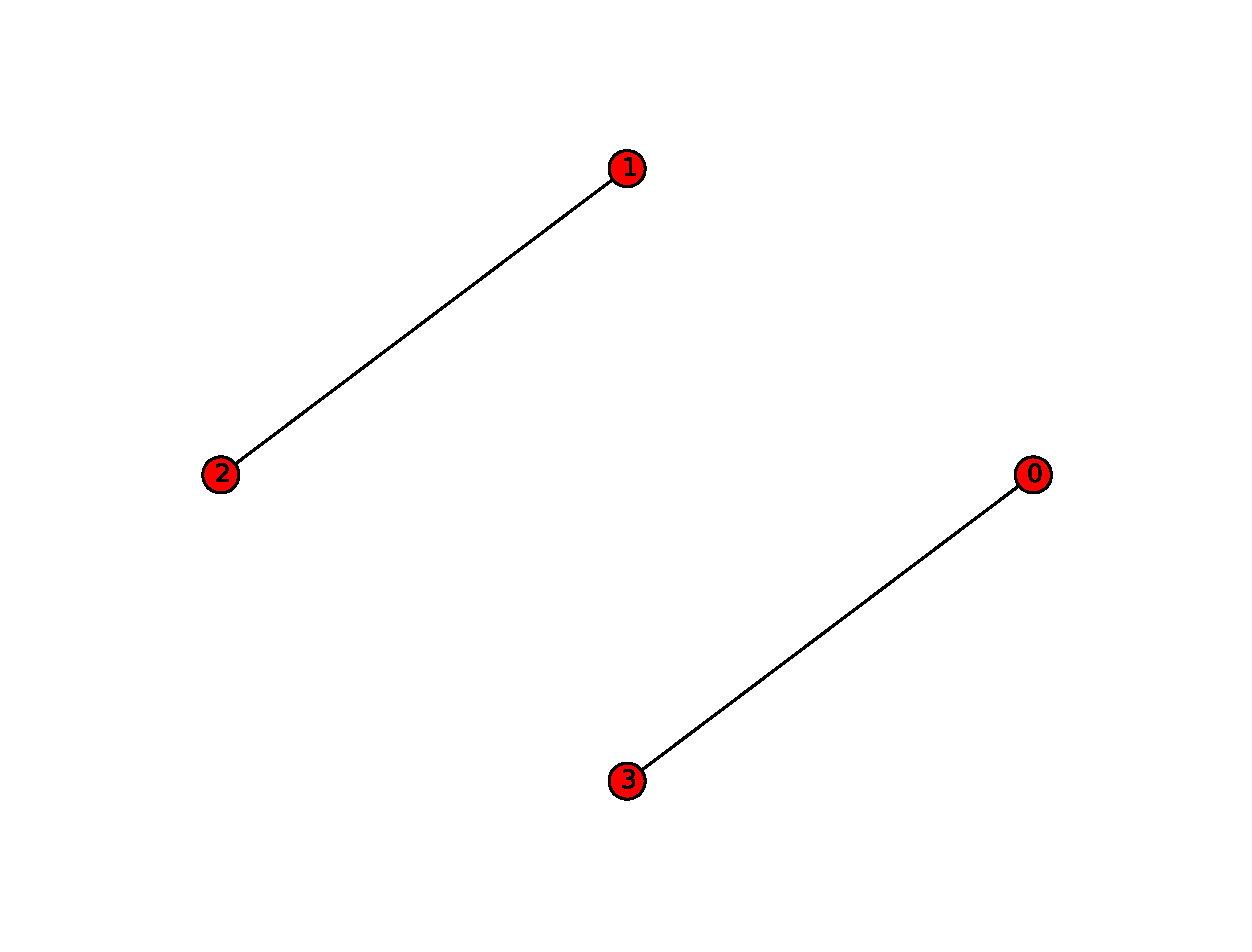
\includegraphics[width=0.32\textwidth]{Figures/G1_swap.eps}  
    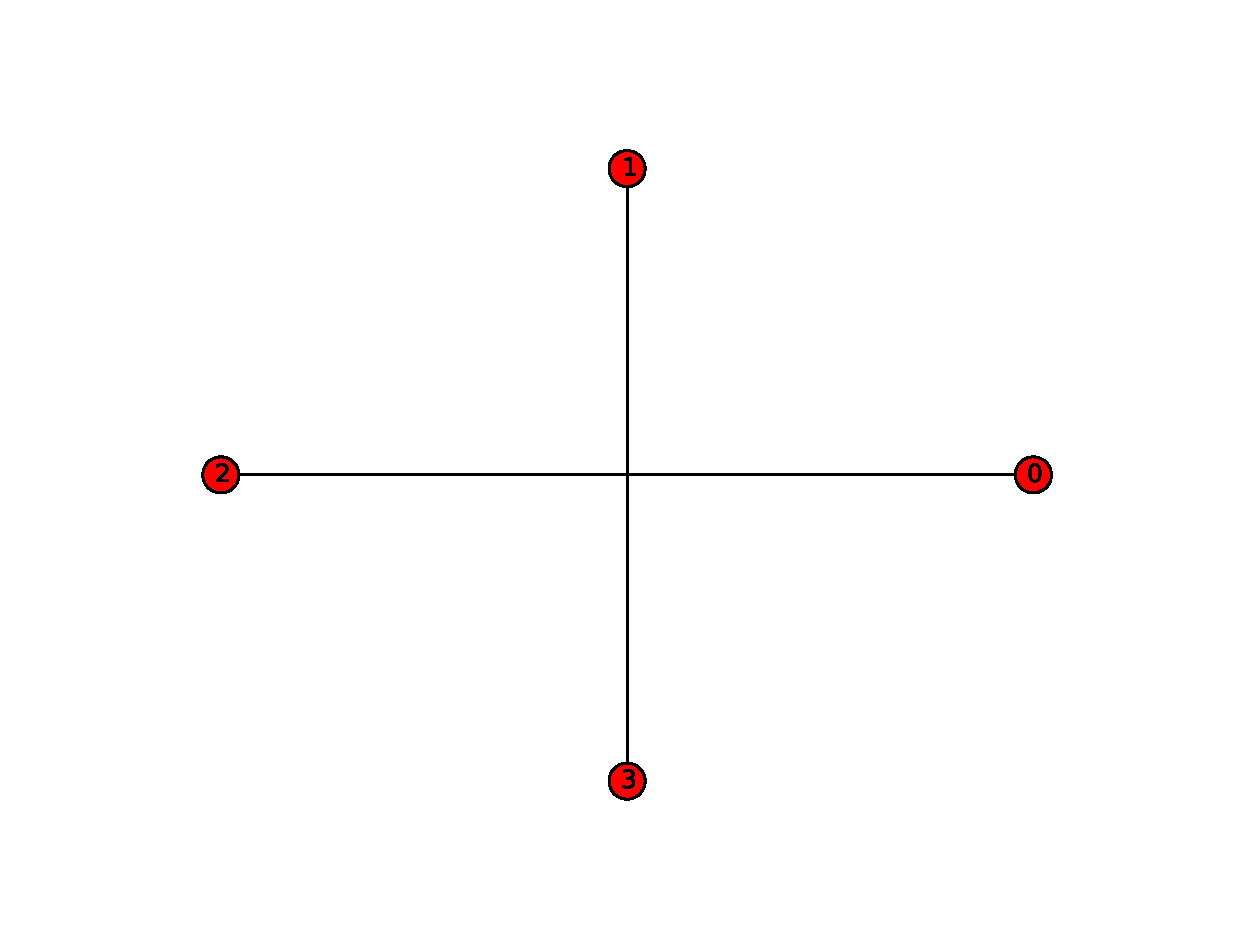
\includegraphics[width=0.32\textwidth]{Figures/G2_swap.eps}  
	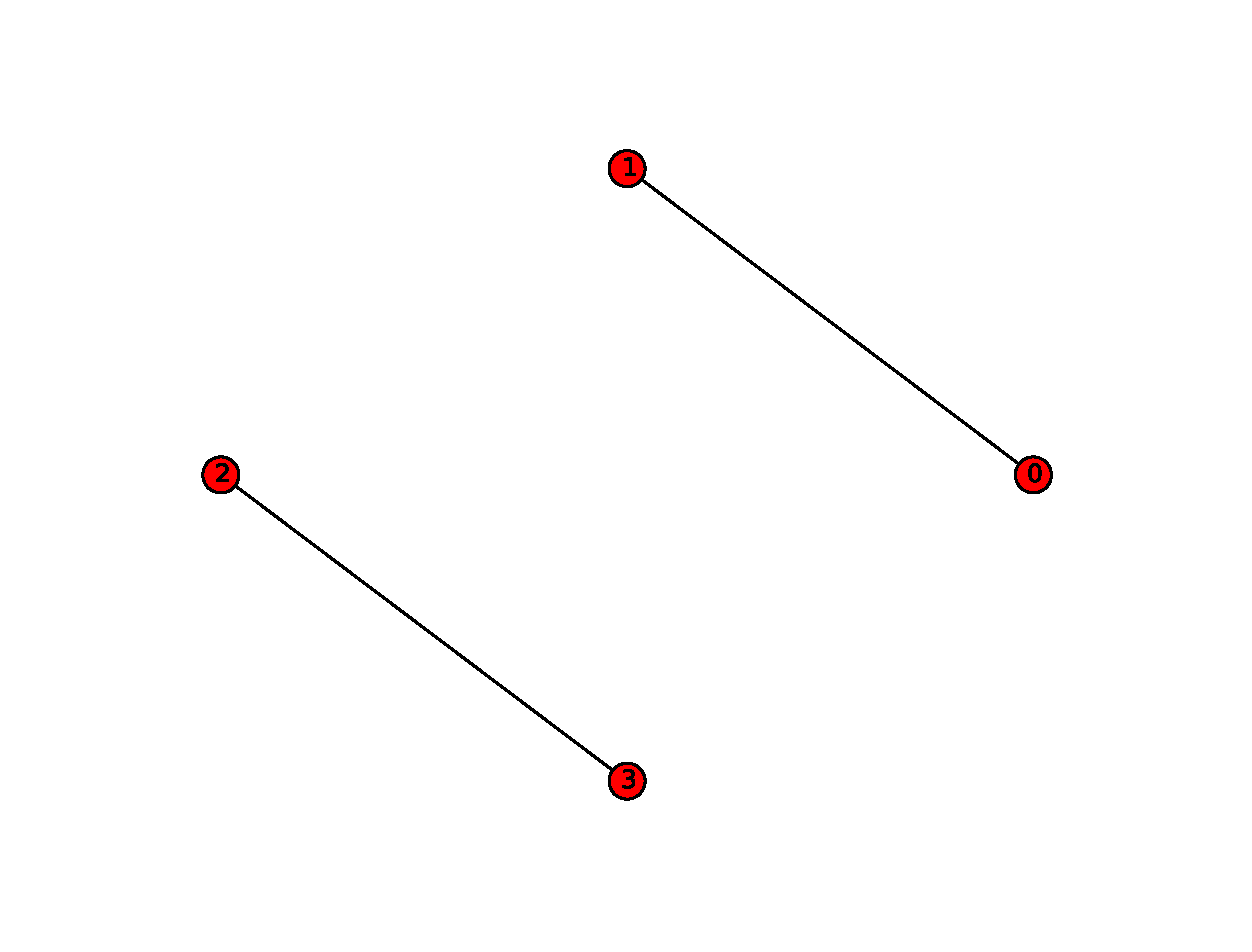
\includegraphics[width=0.32\textwidth]{Figures/G3_swap.eps} 

\end{frame}



\begin{frame}{3.The Randomization Methods}

\footnotesize{Preserved-Degree-Distribution Type Randomization, $p(k)$} 
	\centering	
	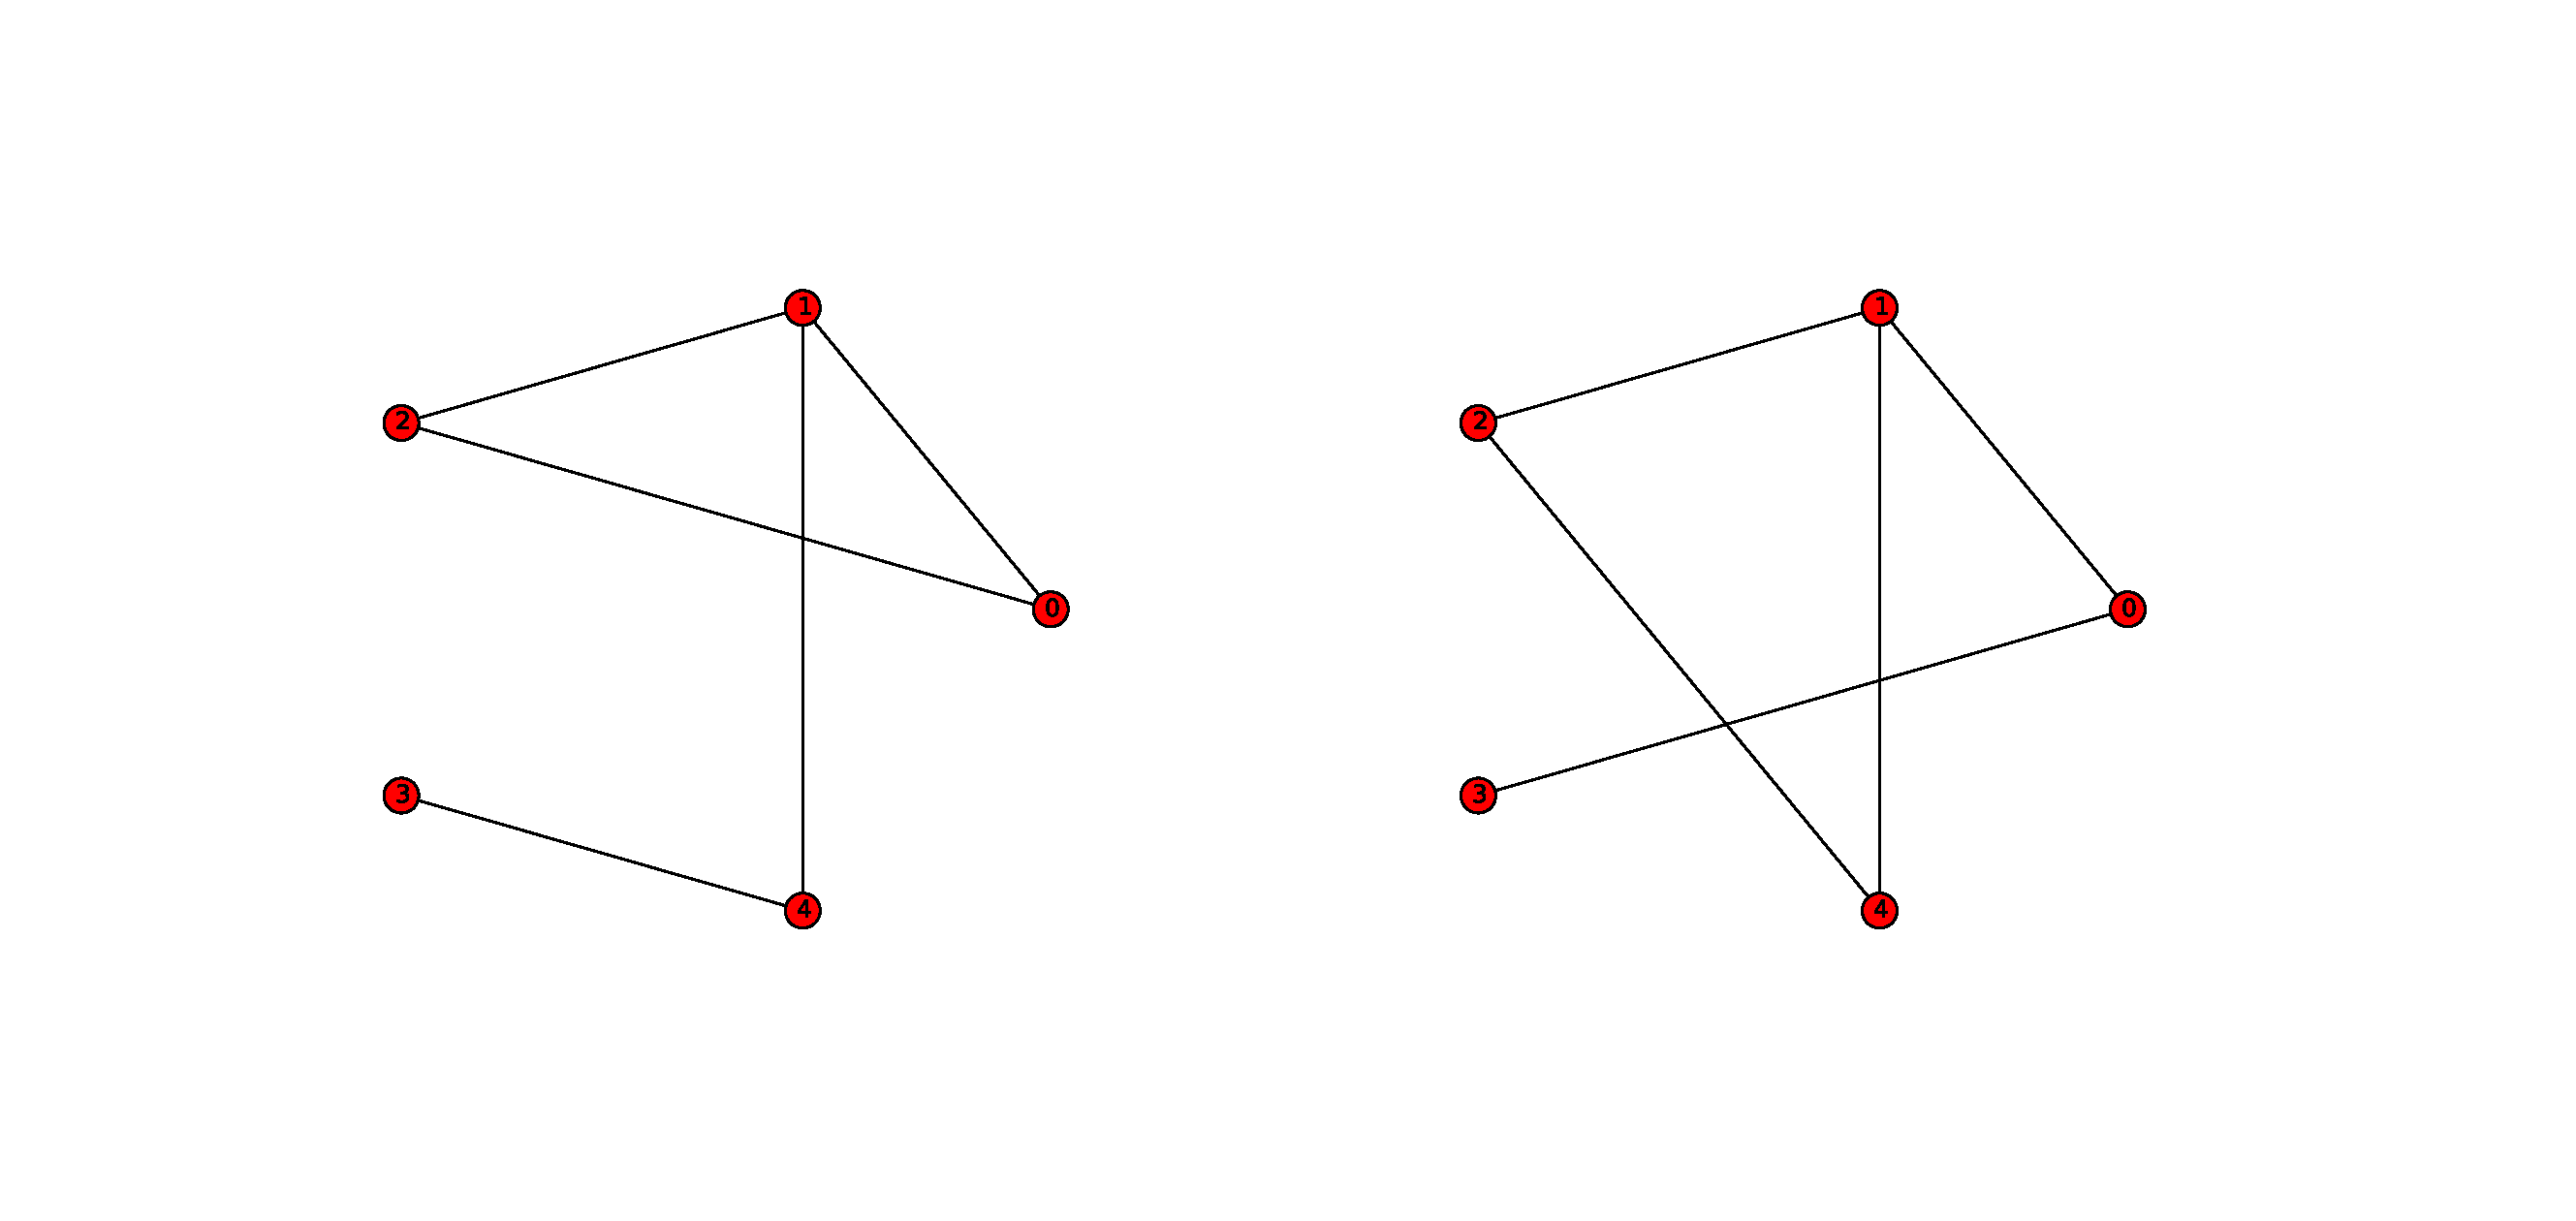
\includegraphics[width=0.8\textwidth]{Figures/G_degree_dist_1.eps}  

 $p(k=1)=\frac{1}{5}$, $p(k=2)=\frac{3}{5}$, and $p(k=3)=\frac{1}{5}$ 

\end{frame}



\begin{frame}{3.The Randomization Methods}

\footnotesize{Configuration Model Randomization} 
	\centering	
	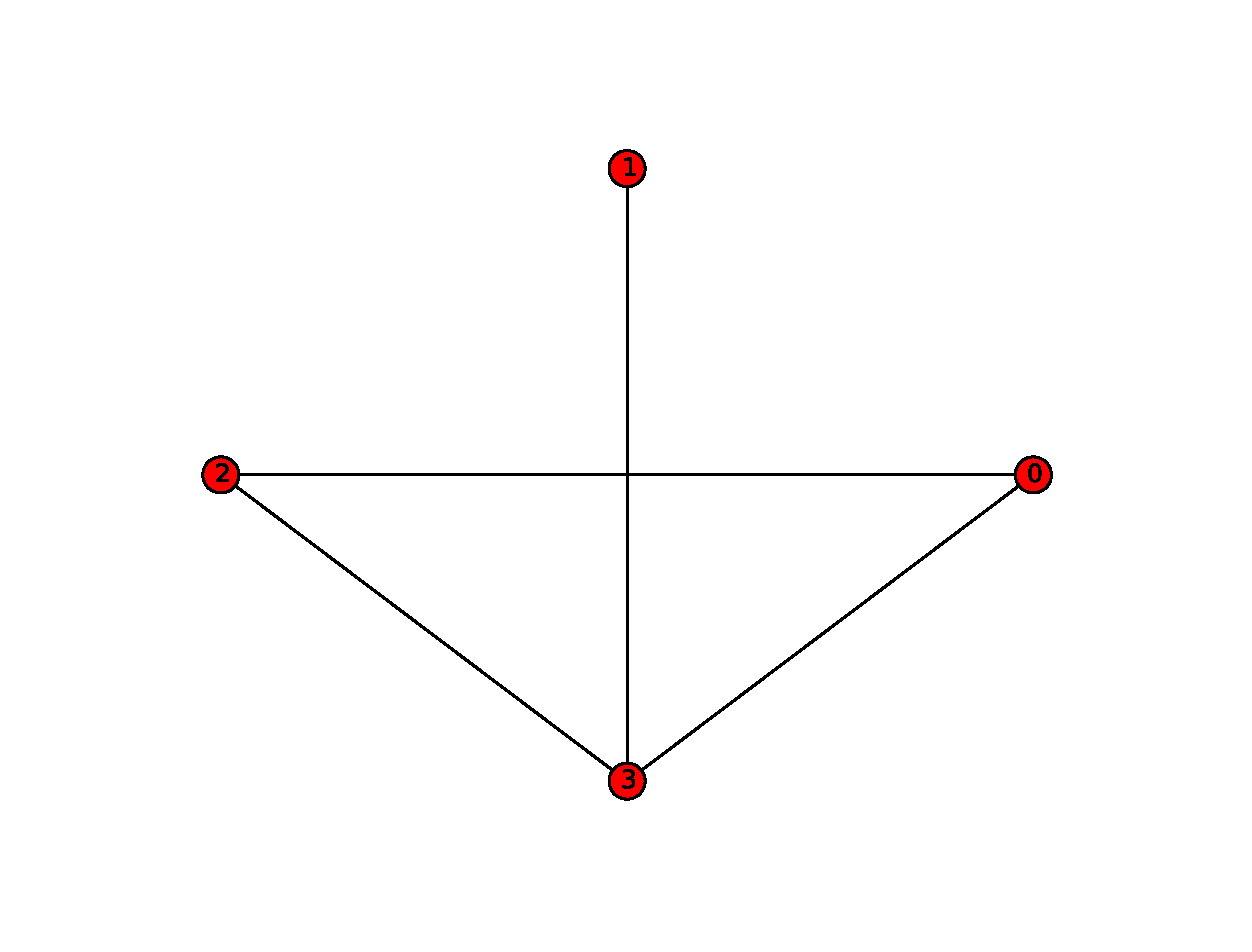
\includegraphics[width=0.3\textwidth]{Figures/G_config_1.eps}  
	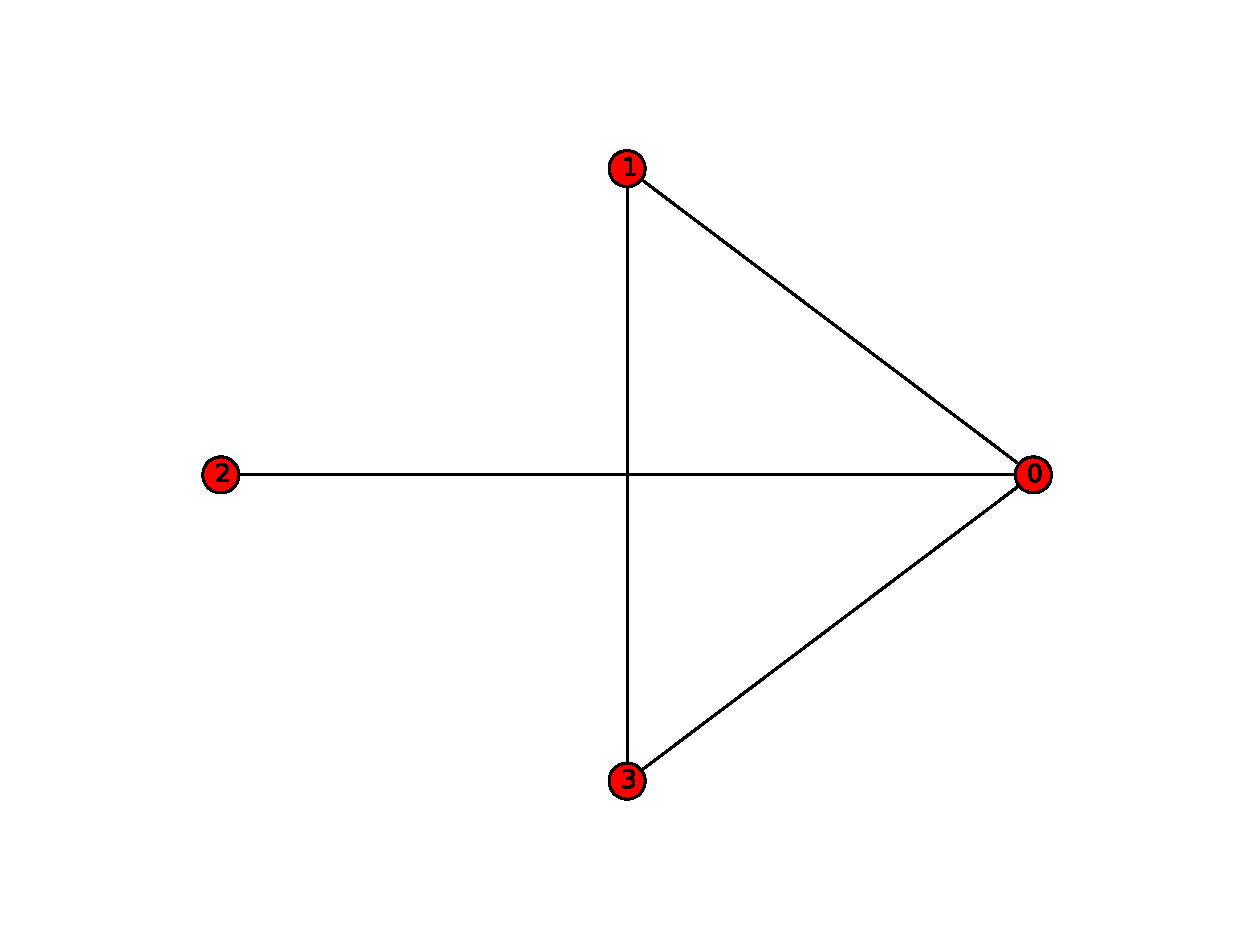
\includegraphics[width=0.3\textwidth]{Figures/G_config_2.eps}  \\
\tiny{(left): $k_0 = 2$, $k_1 =1$, $k_2=2$, $k_3=3$  (right): $k_0 = 3$, $k_1 =2$, $k_2=1$, $k_3=2$. The degree sequence in non-increasing order in both graphs: $\{3,\,2,\,2,\,1\}$ } 
\break

\footnotesize{Partial Randomization}

\includegraphics[width=0.8\textwidth]{Figures/p1.png}  

\end{frame}



\begin{frame}{4.Network Characterizations}

{Network Density, $\kappa=\frac{2L}{N(N-1)}$} 
\break
\break
\footnotesize{FCM related graphs ~~~~~~~~~~~~~ ACM related graphs}
	\centering	
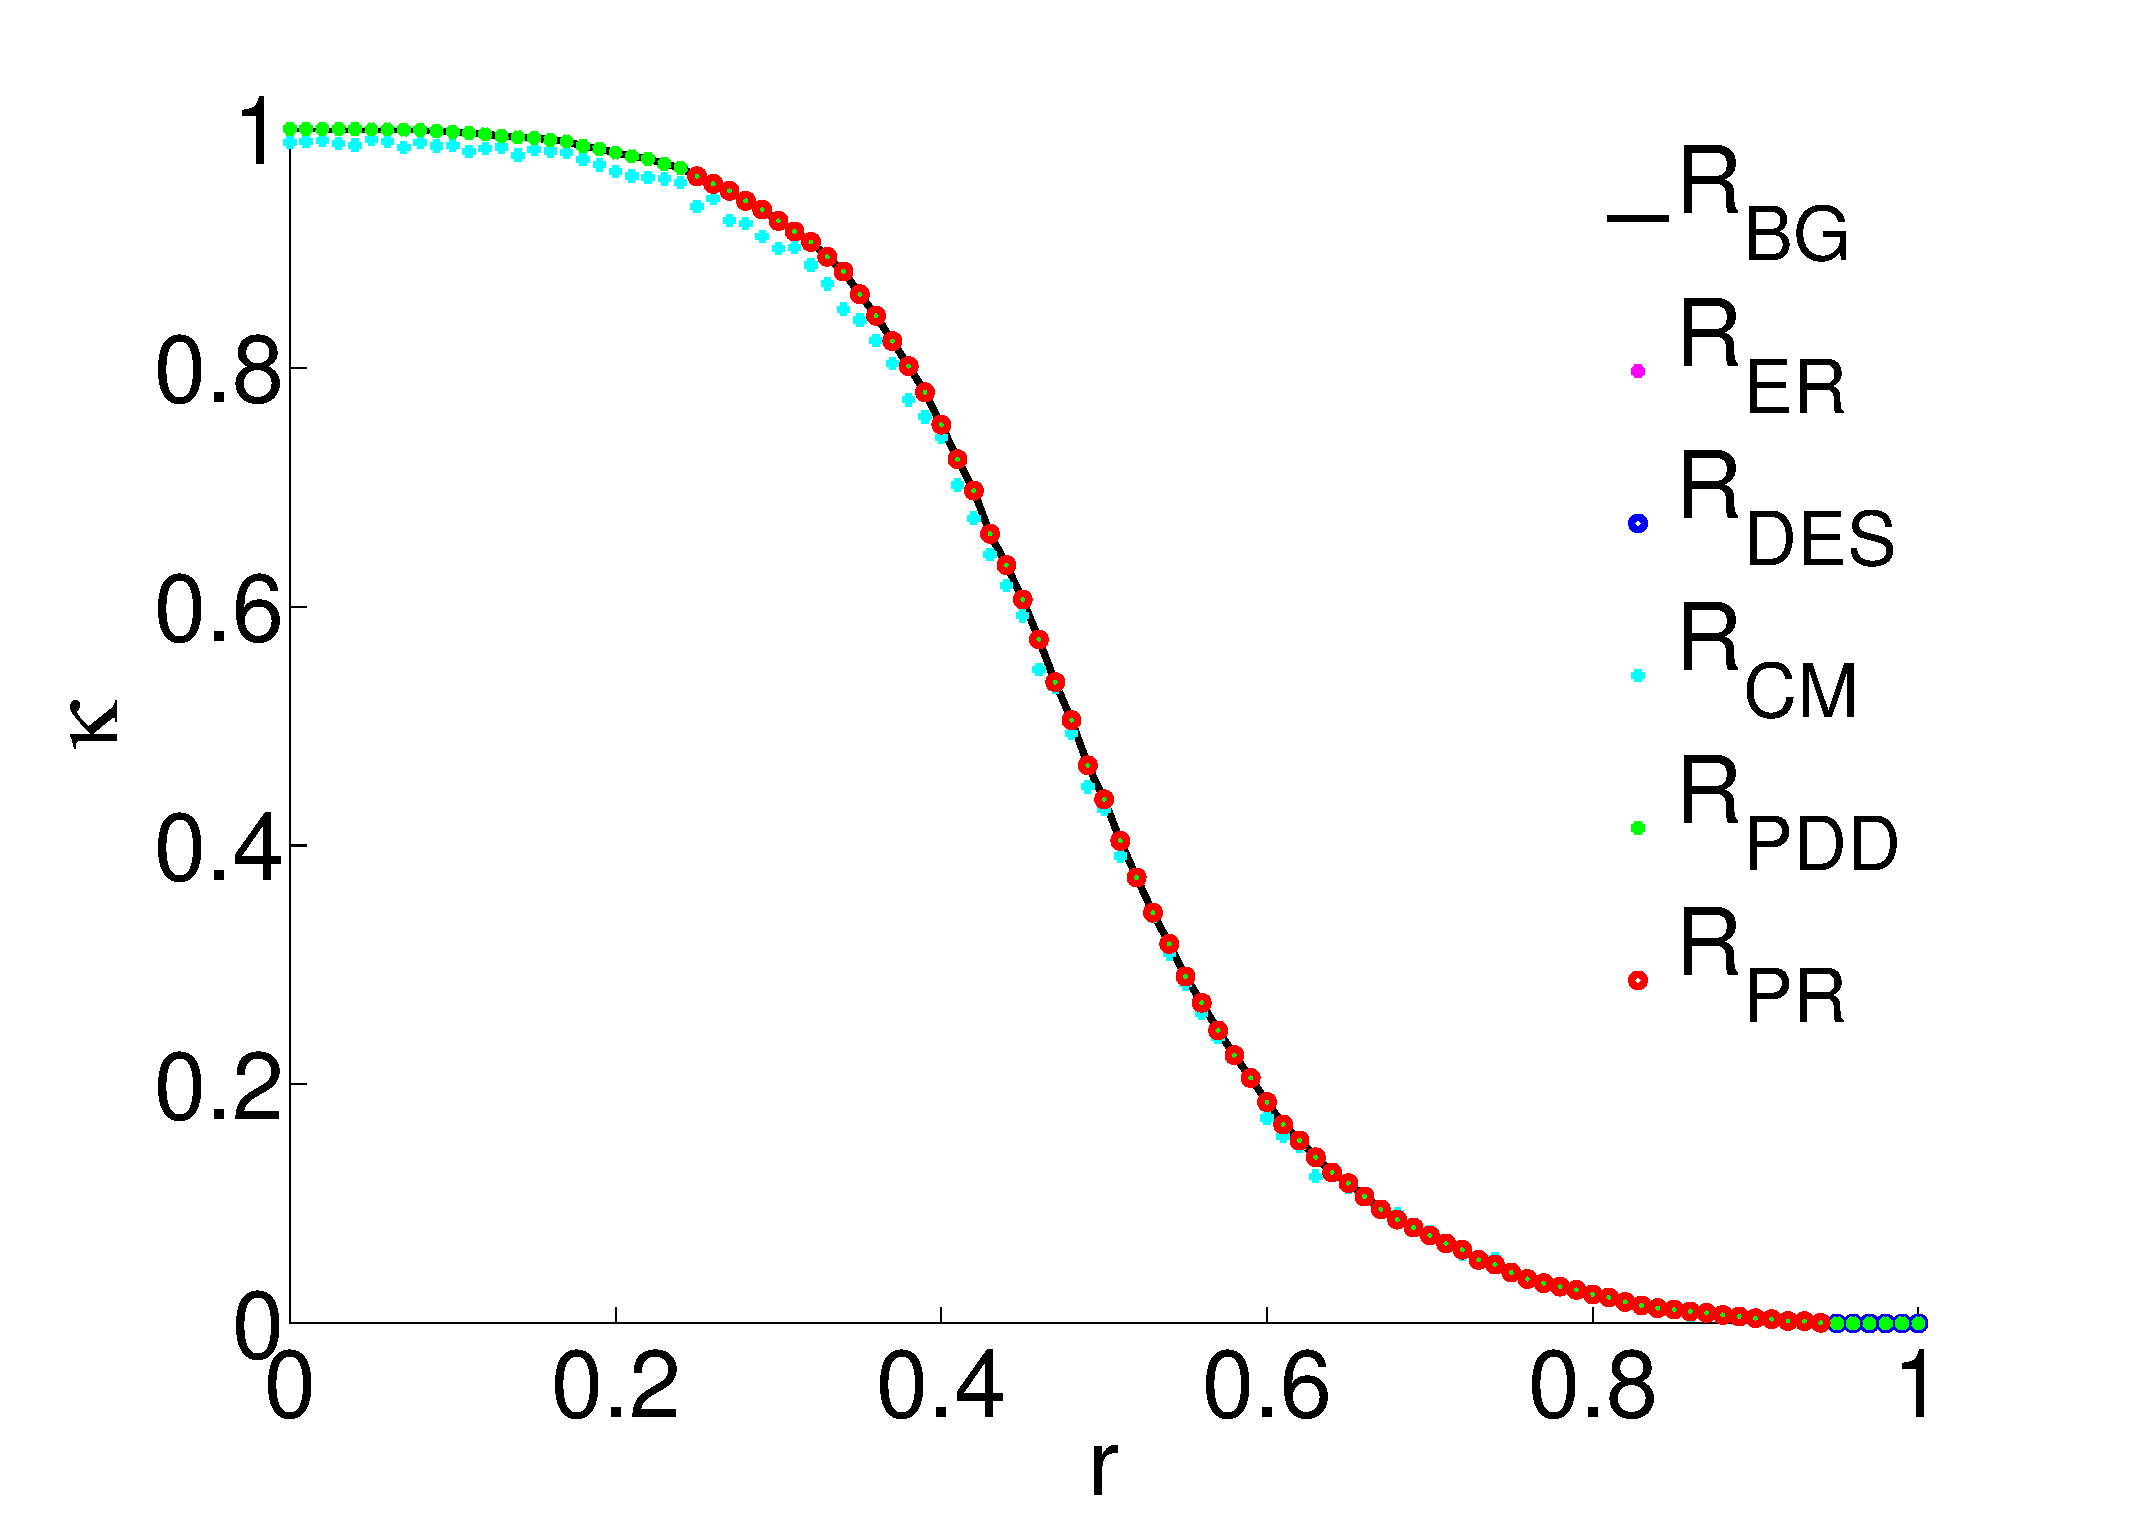
\includegraphics[width=0.40\textwidth]{Figures/Network_Density_Fnc.eps}
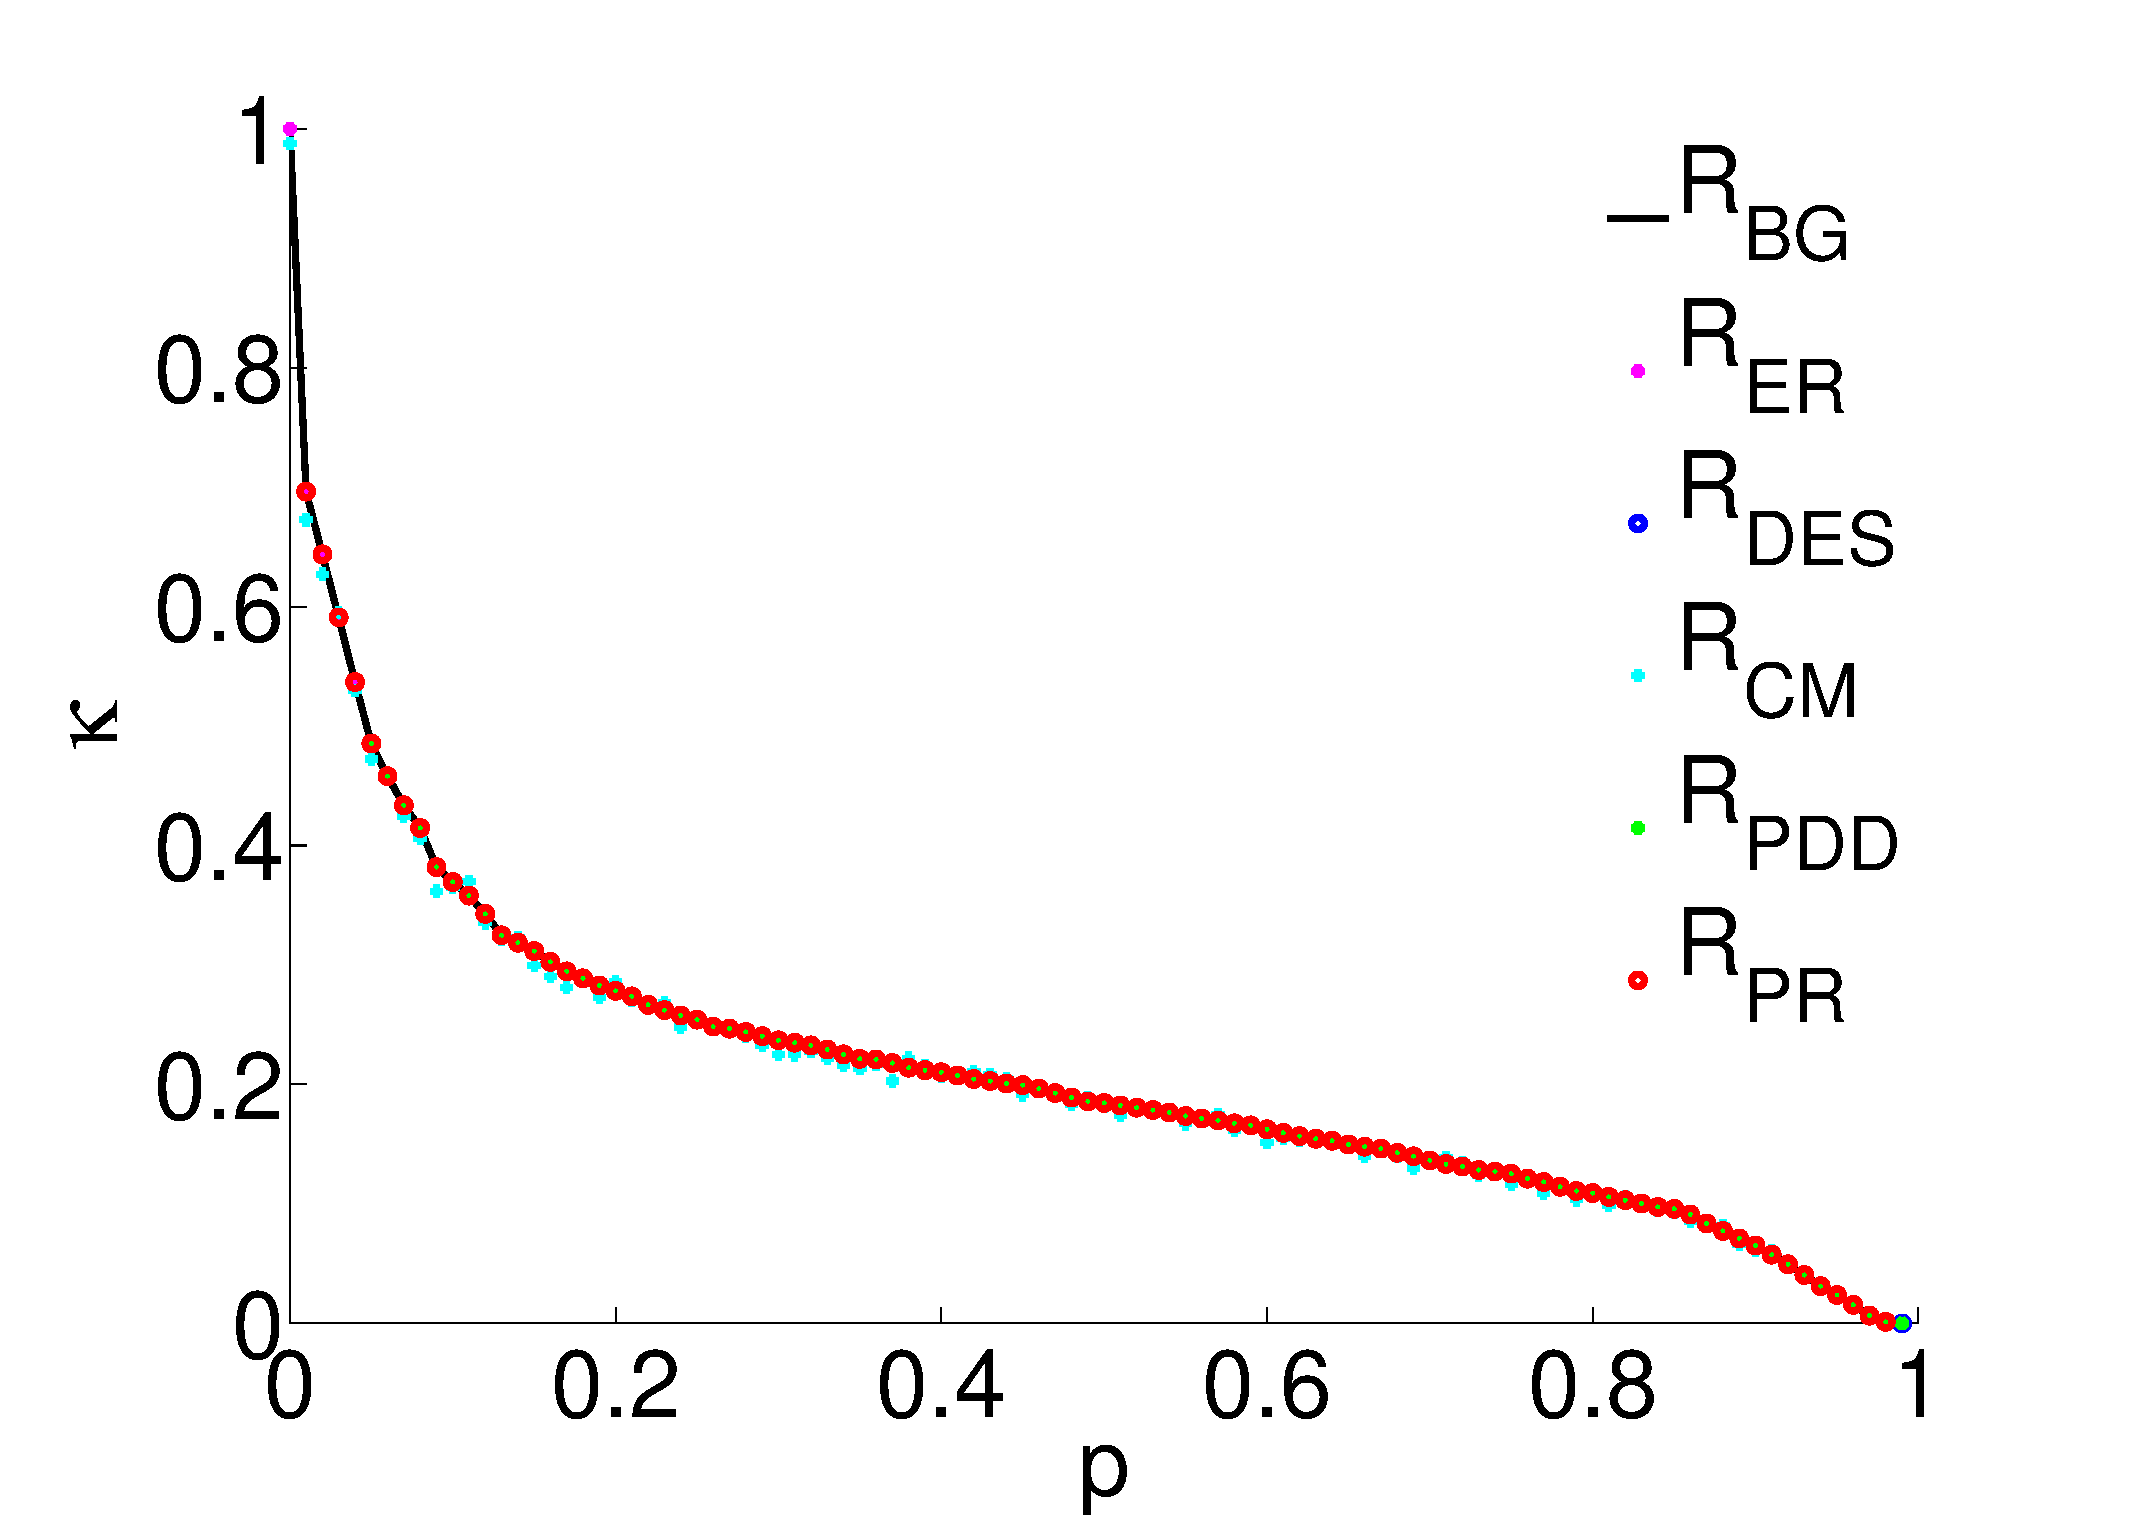
\includegraphics[width=0.40\textwidth]{Figures/Network_Density_Stru.eps} 

\end{frame}






\begin{frame}{4.Network Characterizations}

{Transitivity,  $T = \frac{2\sum\limits_{i \epsilon N}  t_i}{\sum\limits_{i \epsilon N}k_i (k_i - 1)}$ } 
\break
\break
\break
\footnotesize{FCM related graphs ~~~~~~~~~~~~~ ACM related graphs}
	\centering	
    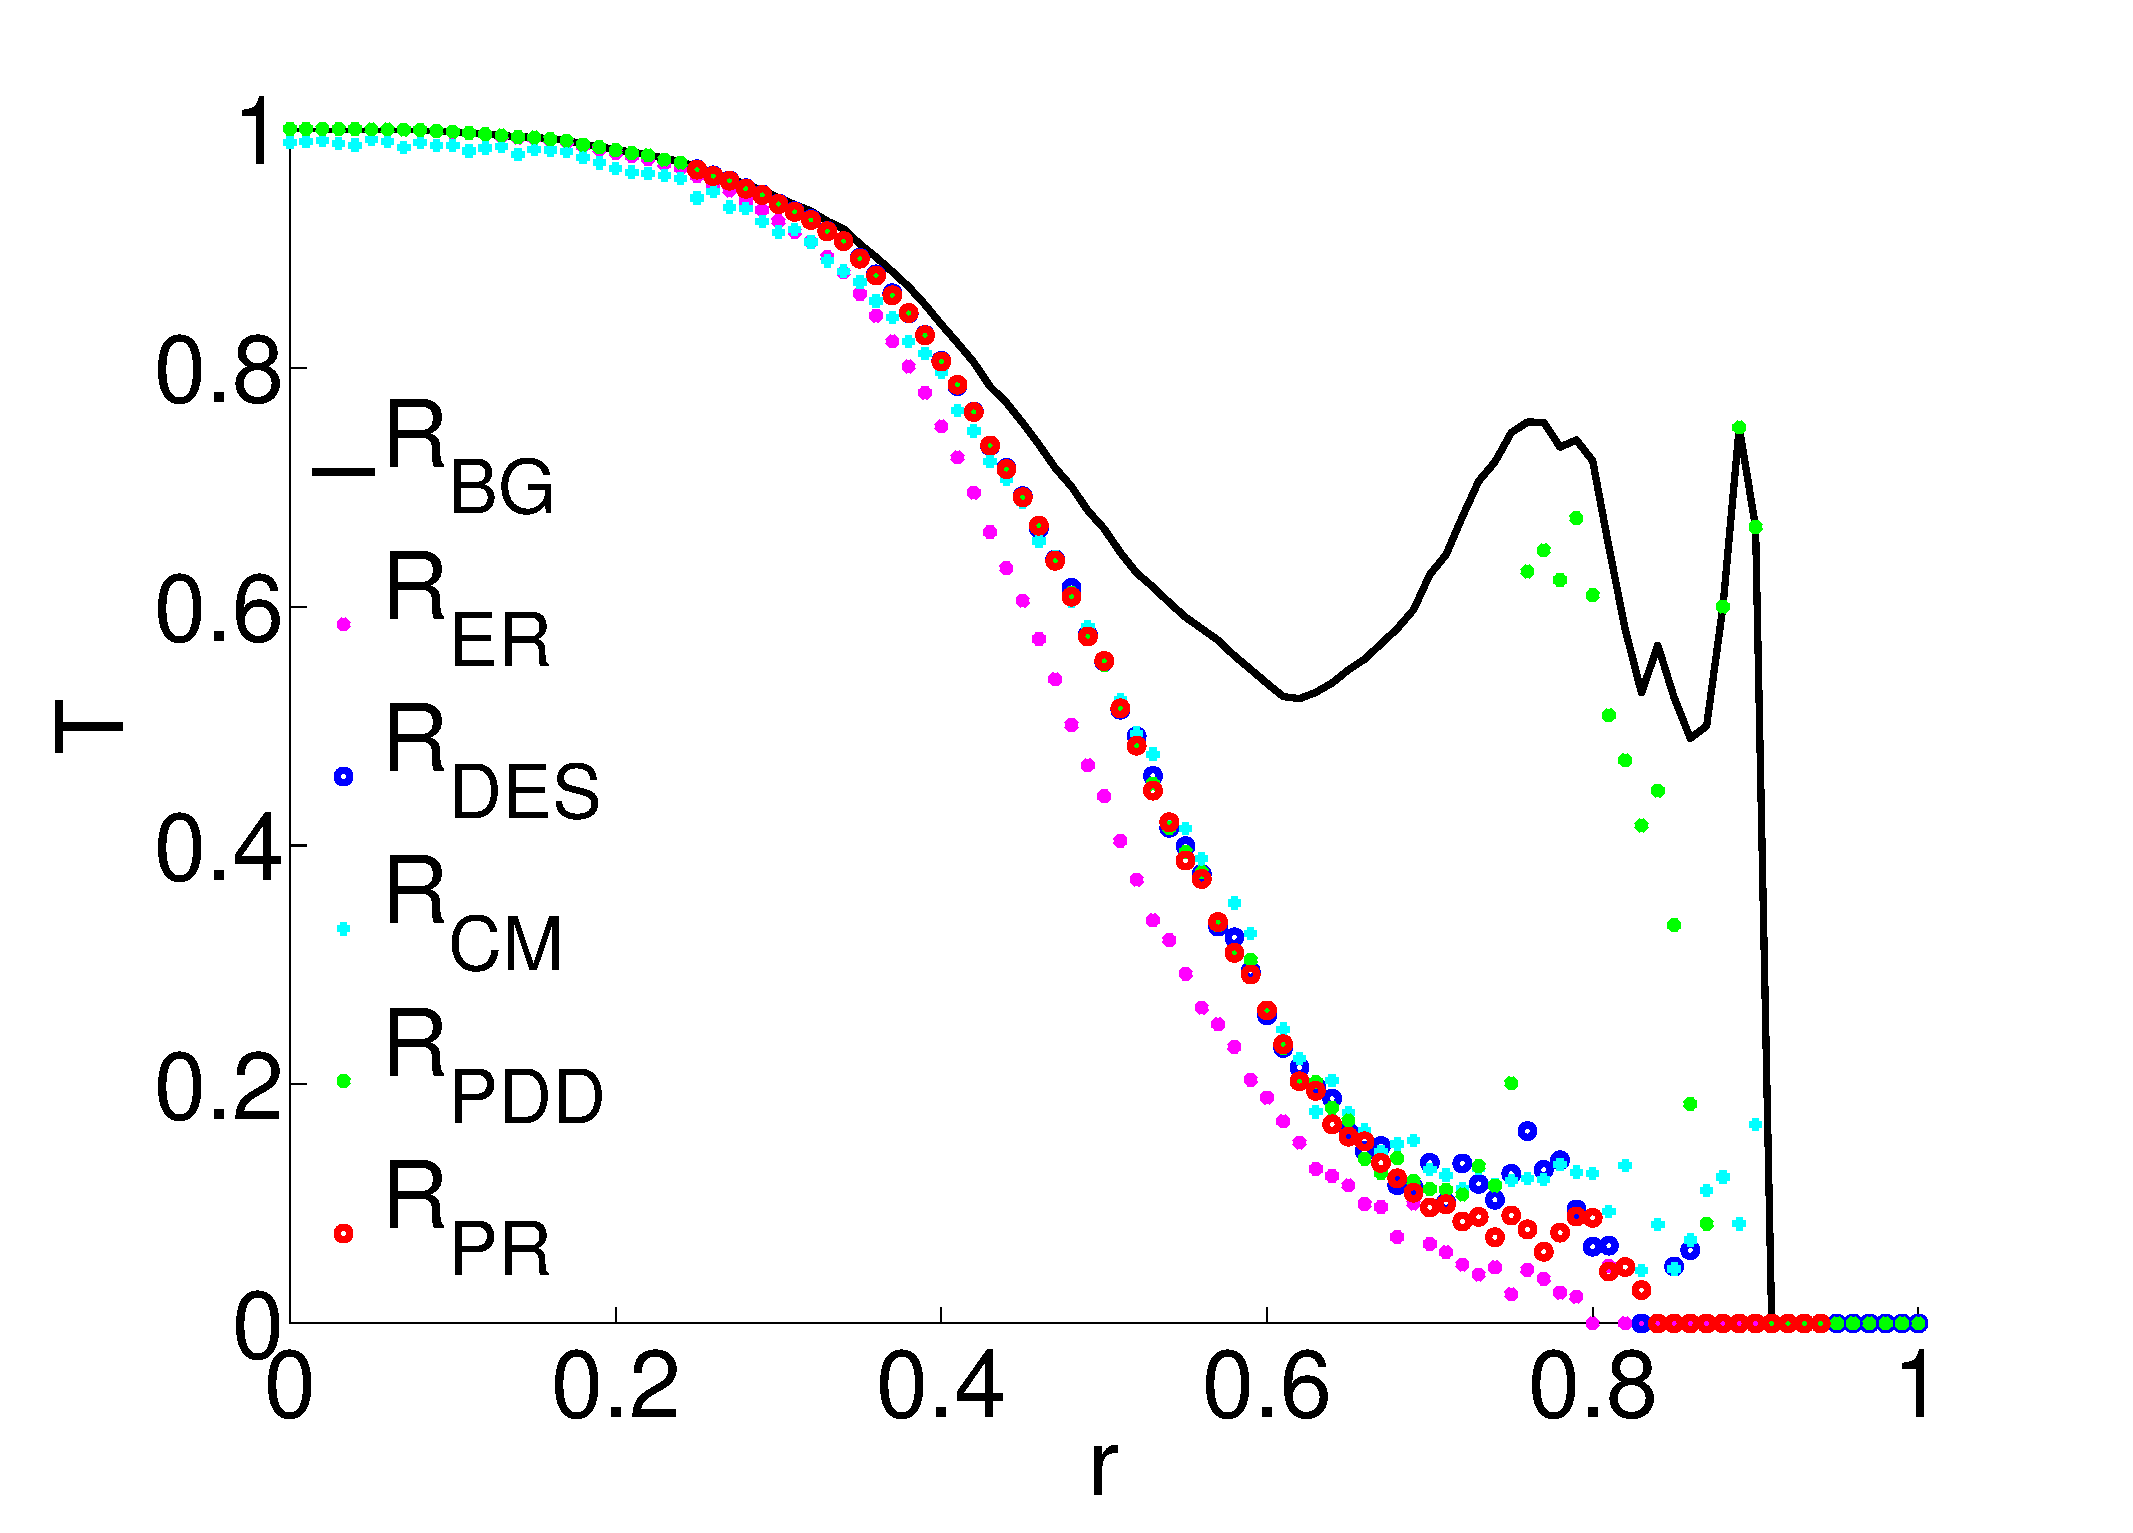
\includegraphics[width=0.40\textwidth]{Figures/Transitivity_Fnc.eps}
	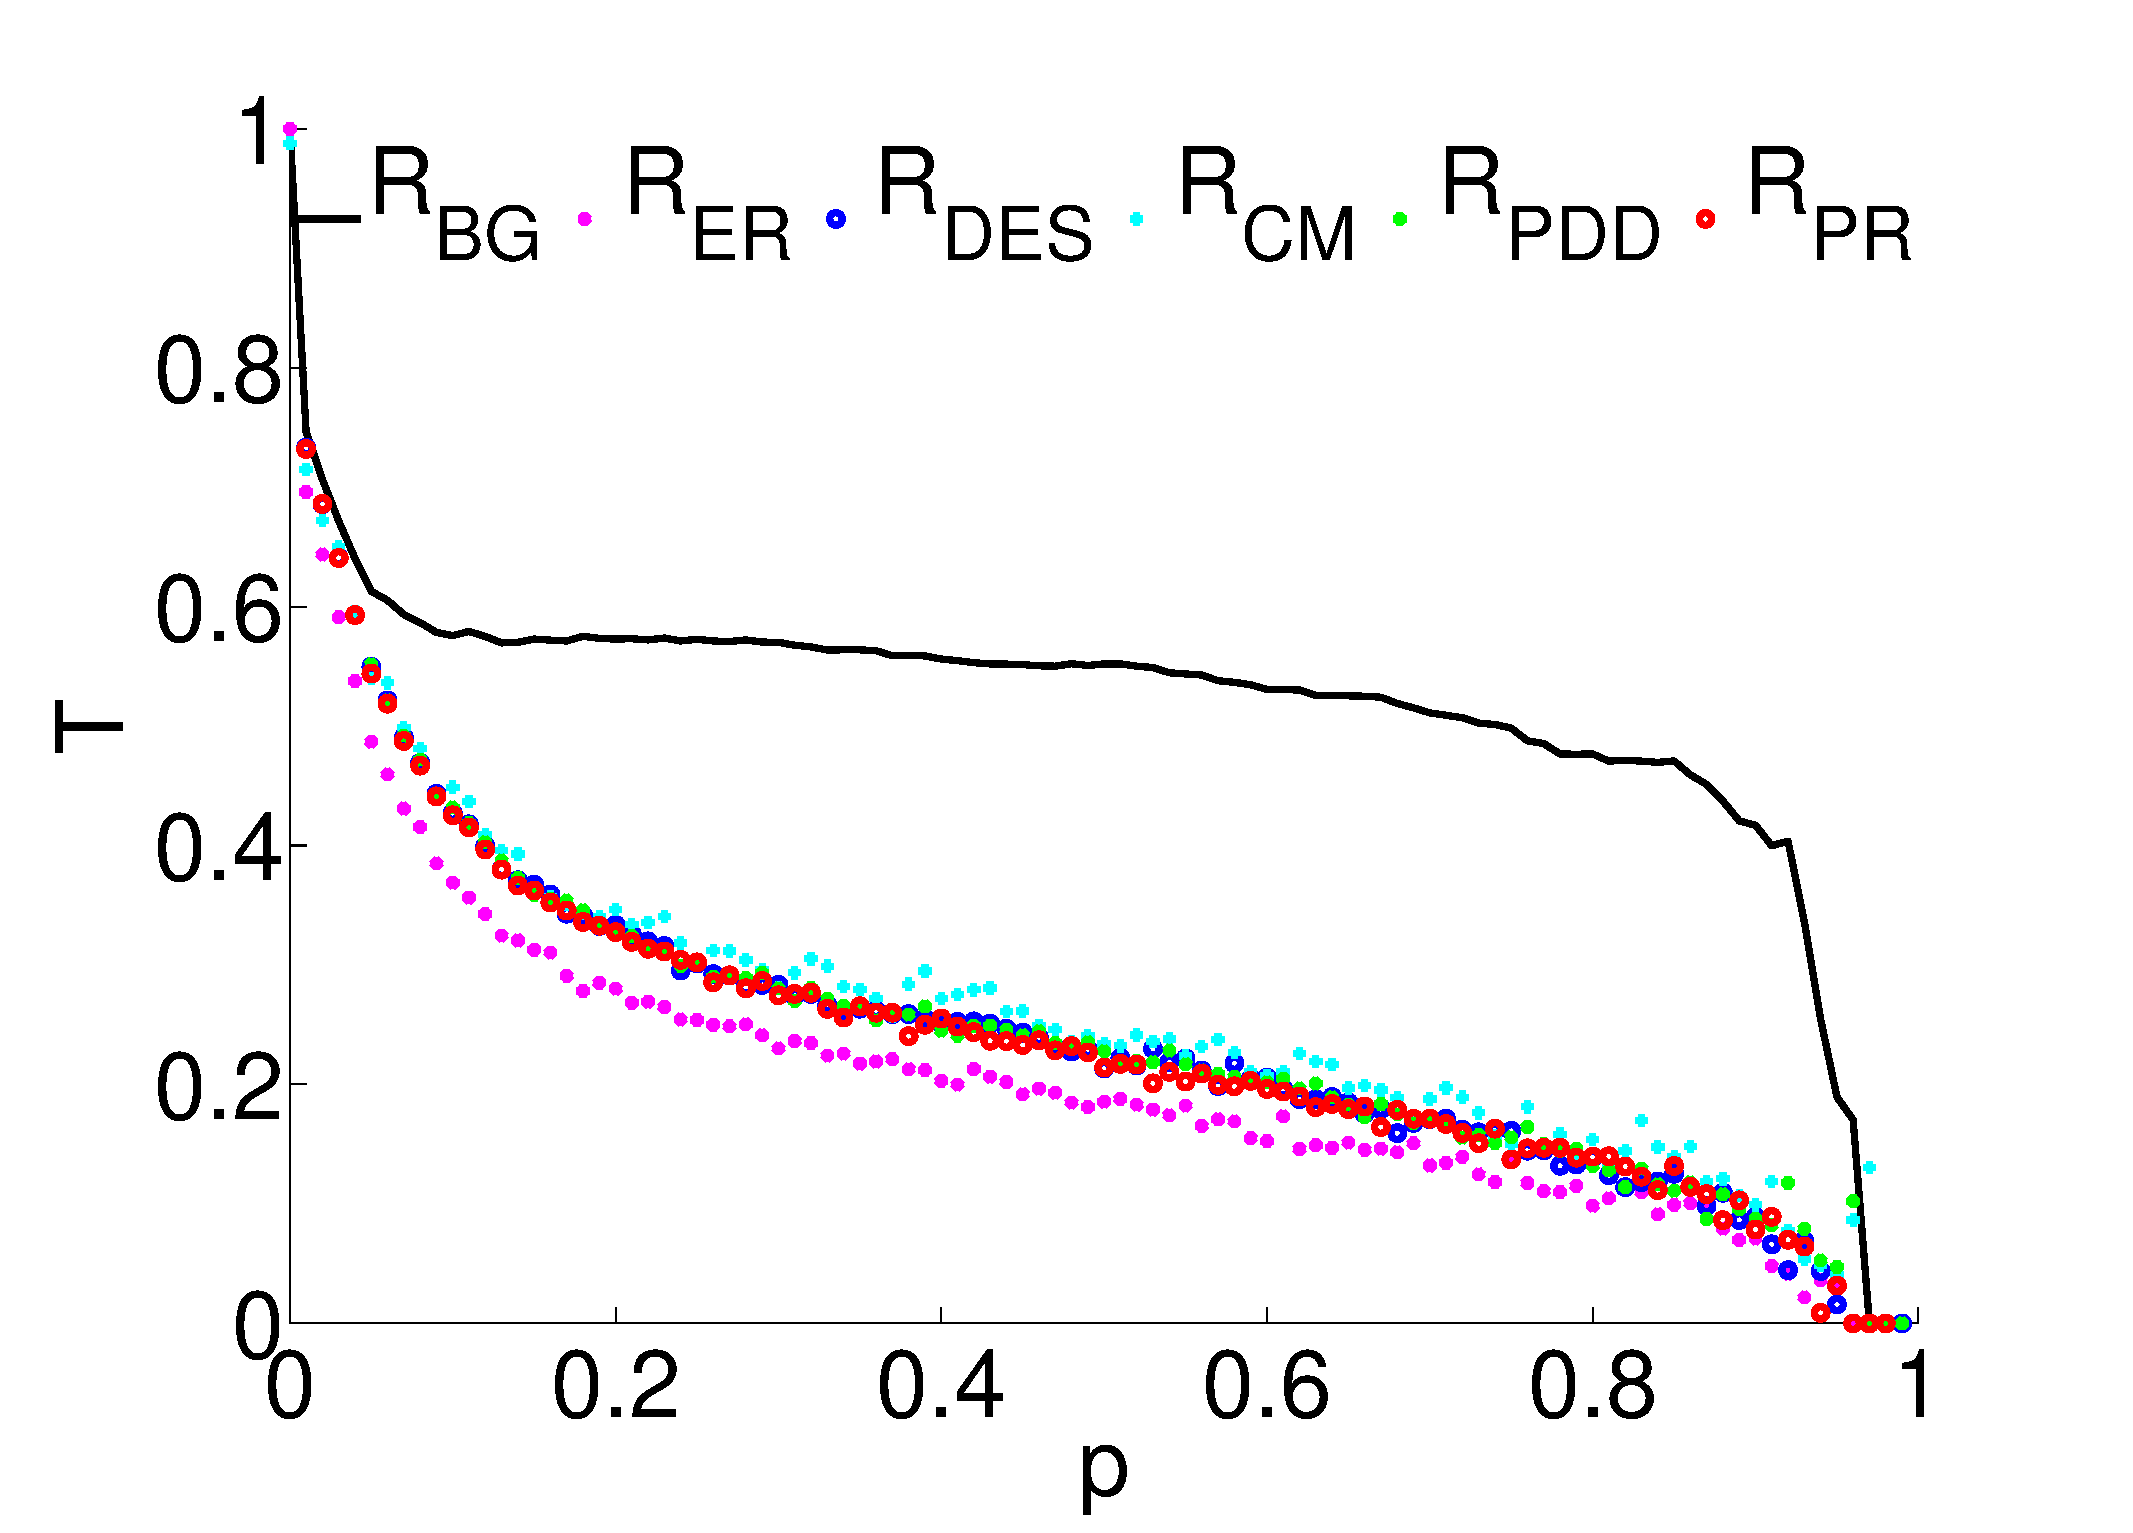
\includegraphics[width=0.40\textwidth]{Figures/Transitivity_Stru.eps} 
	
\end{frame}




\begin{frame}{5.Neuronal Activity Model}
\footnotesize{FitzHugh-Nagumo Oscillations, Local Dynamics with Gaussian White Noise Source }

\begin{subequations}
\begin{align}\dot{x} = \tau \left( y + \gamma x - \frac{x^3}{3} \right) + Dn_x  \label{eqn: frobenius 1}\\  \dot{y} = -\frac{1}{\tau} (x - \alpha + b y ) + Dn_y , \label{eqn: frobenius 2 }   \end{align} 
\end{subequations}

 \centering
 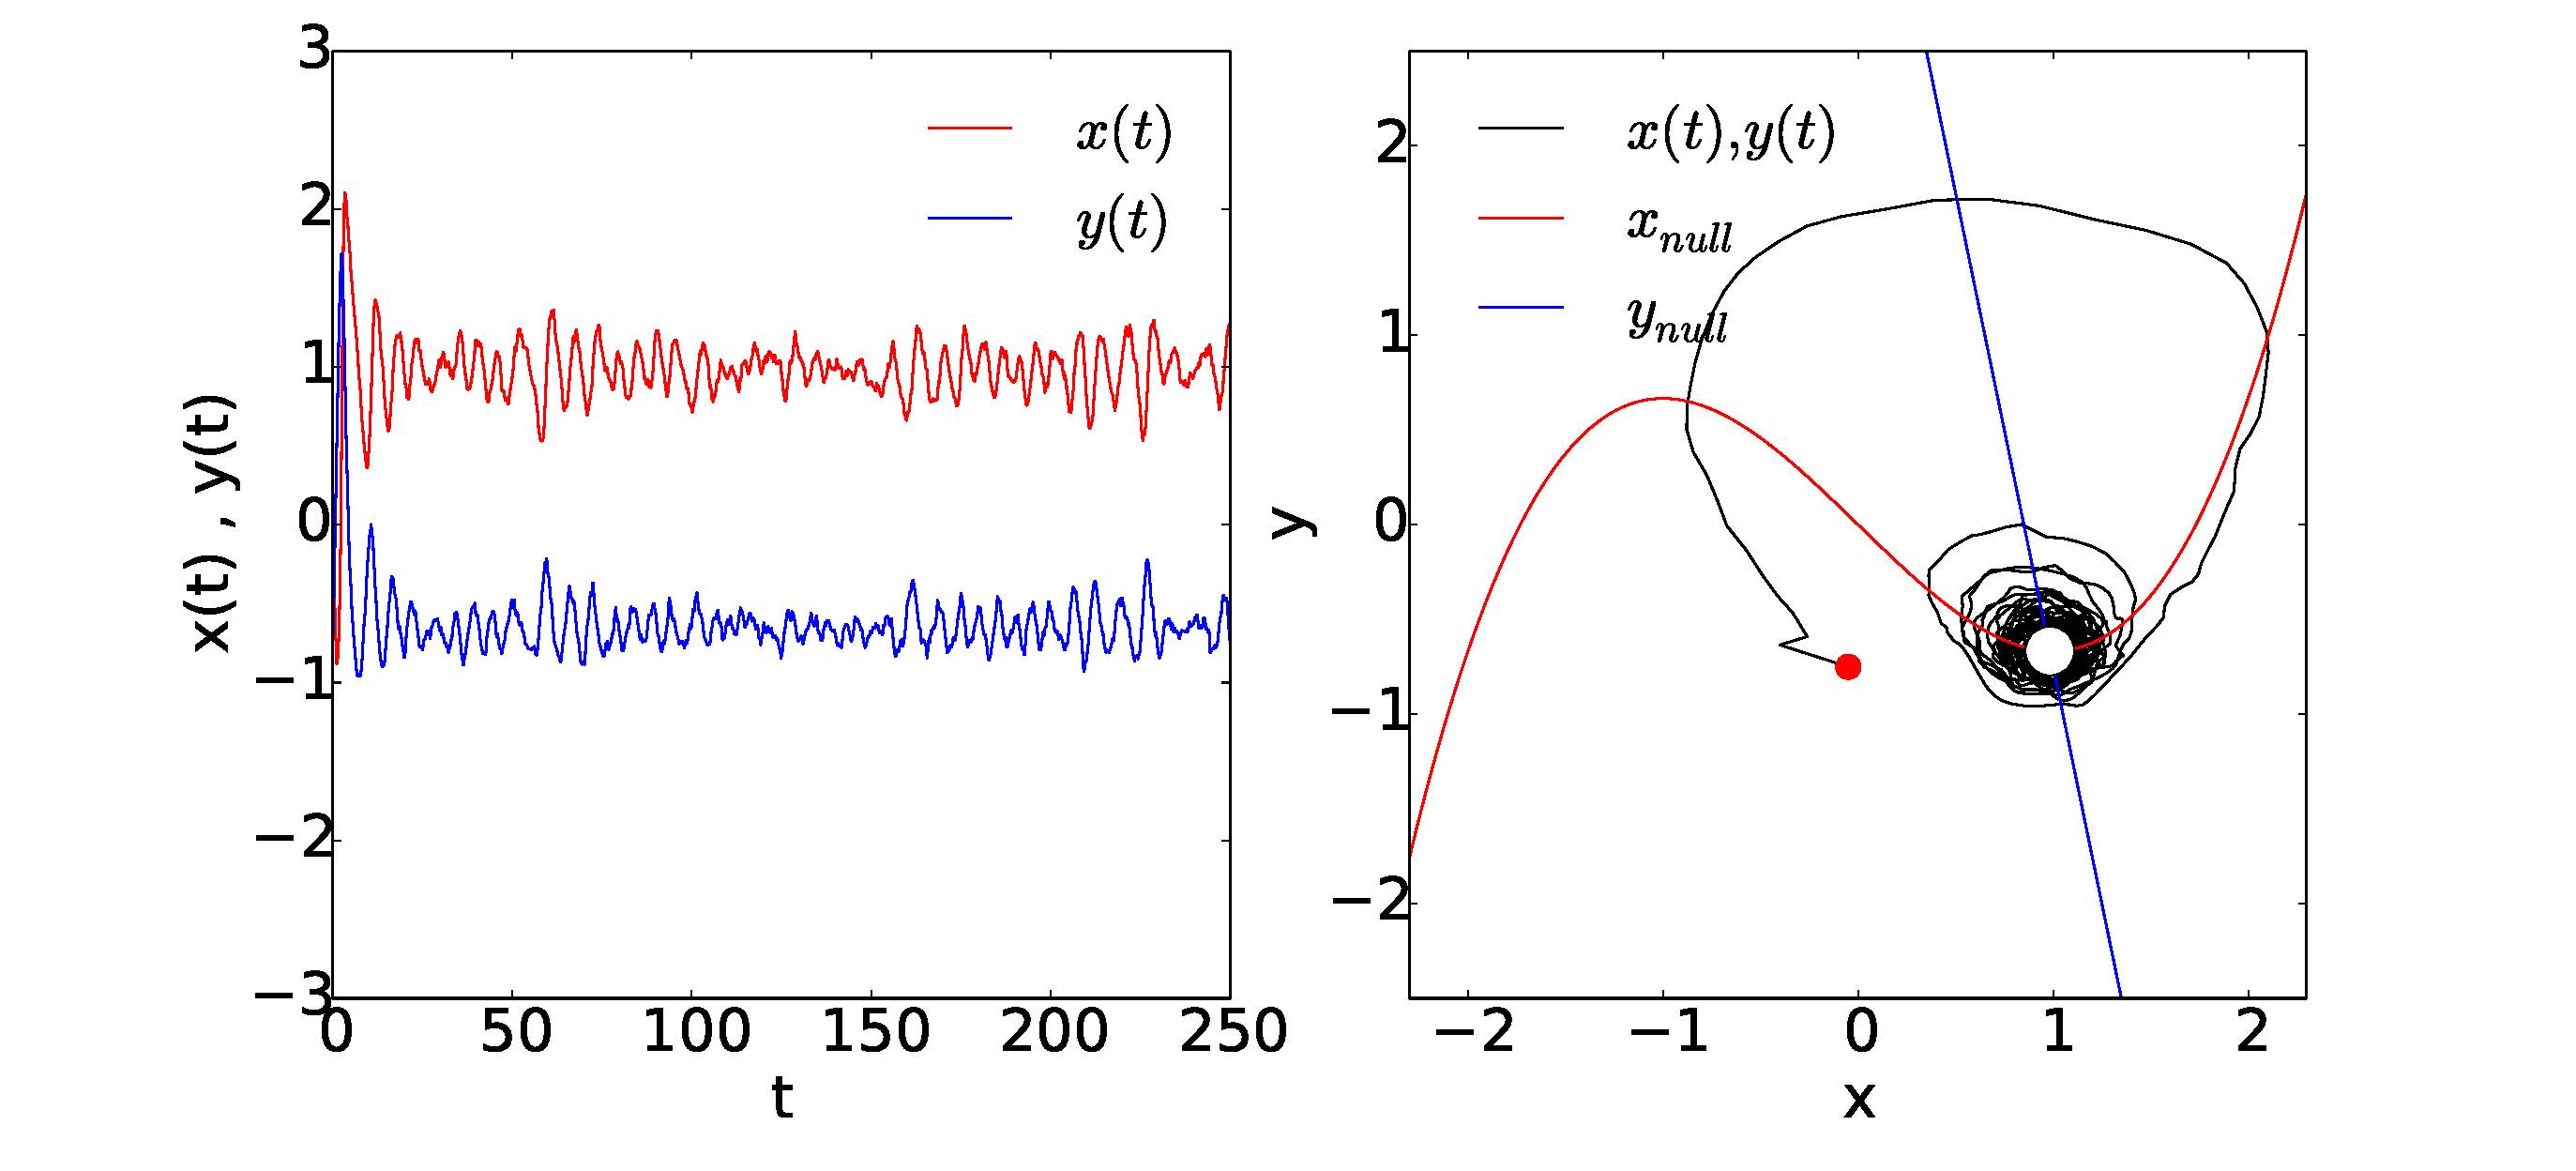
\includegraphics[width=0.9\textwidth]{Figures/FHN_noise.eps}

\end{frame}









\begin{frame}{Research Proposals}
\footnotesize{\textit{i)How does functionally correlated behavior among cortical and subcortical brain regions emerge from the structural connectivity? }} 
\break
\break
\footnotesize{\textit{ii)Does the topological properties as well as temporal dynamics of the brain graph differ from that of random graphs? }}

\centering
\includegraphics[width=0.6\textwidth]{Figures/presi_1.eps} 

\end{frame}


\begin{frame}{7.Results}
\footnotesize{Neuronal Activity Simulations of FCM Related Brain Graphs to fMRI-BOLD Data} 
\break
\break
\break
\centering
    \includegraphics[width=0.40\textwidth]{Figures/PA_FCM_c_02.eps} 
	\includegraphics[width=0.40\textwidth]{Figures/PA_FCM_v_7.eps} 
	
\end{frame}




\begin{frame}{7.Results}
\footnotesize{Neuronal Activity Simulations of ACM Related Brain Graphs to DW-MRI Data} 
\break
\break
\break
\centering
    \includegraphics[width=0.40\textwidth]{Figures/PA_ACM_c_03.eps} 
	\includegraphics[width=0.40\textwidth]{Figures/PA_ACM_v_6.eps} 
	
\end{frame}


\begin{frame}{7.Results}
\footnotesize{Neuronal Activity Simulations of ACM Related Brain Graphs to DW-MRI Data} 
	\centering
	 \includegraphics[width=0.35\textwidth]{Figures/cor_ACM_sim.eps}  
   	 \includegraphics[width=0.35\textwidth]{Figures/cor_ACM_exp.eps} \\
    \centering
    \includegraphics[width=0.7\textwidth]{Figures/cor_ACM_sim_no_best.eps}\\ 
	\centering    
    \includegraphics[width=0.7\textwidth]{Figures/cor_ACM_sim_no_worst.eps} 


	\tiny{$\rho_{43,31}=0.86$, ~~~~~~ $\rho_{90,83}=0.15$}	
	
	
\end{frame}




\begin{frame}{7.Results}
\footnotesize{Comparing BOLD Simulations of Anatomical Brain Graphs to fMRI-BOLD Data} 
\break
\break
	\centering
	 \includegraphics[width=0.8\textwidth]{Figures/cor_BOLD_ACM_sim_no_best.eps} \\
   	 \includegraphics[width=0.8\textwidth]{Figures/cor_BOLD_ACM_sim_no_worst.eps} 

  \tiny{ $\rho_{58,59}=0.48$ ~~~~~~~ $\rho_{90,89}=0.11$ }
\end{frame}





\begin{frame}{7.Results}
\footnotesize{How to Compare the Modeled Temporal Dynamics of Brain Graphs to that of the Random Networks ? }

\begin{itemize}
  \item construct brain graphs and their random networks at defined $r$- and $p$-ranges for FCM and ACM based empirical data  
  \item extract FHN network modeled time-series in each graph
  \item find Pearson correlation coefficients $\rho$ between pairwise combination of $N=90$ nodes in each graph
  \item distribute $\rho$ values in histograms for each graph
  \item compare histograms via Bhattacharya coefficients :
    \end{itemize}
\begin{equation}
d(H_b, H_r) = \sqrt{1- \dfrac{1}{ \sqrt{\bar{H_r} \bar{H_b} N^2}} \sum_{i} \sqrt{H_r(i)H_b(i)} } 
\end{equation}

\end{frame}




\begin{frame}{7.Results}
\footnotesize{Comparison of ACM Related Brain Graph to the Random Networks}

\includegraphics[width=0.78\textwidth]{Figures/Random_ACM_PA.eps}

\end{frame}




\begin{frame}{7.Results}
\footnotesize{Comparison of ACM Related Brain Graph to the Random Networks}

\includegraphics[width=0.8\textwidth, height = 7cm]{Figures/Random_ACM_histo.eps}

\end{frame}


\begin{frame}{8.Future Directions}
bla
\end{frame}




\end{document}



